\chapter{Results}

\section{Workshop Study}
The workshop study had 8 participants, 6 of whom reach the finished garment stage and fit evaluation (Figure \ref{fig:workshop_garments}). All participants used a 150 cm bolt.

They had a mean maximum bodice circumference of 99.96 cm, median of 98.50 cm and a standard deviation of 8.00 cm (Figure \ref{fig:workshop_max_circ}). The mean shirt length was 60.36 cm, median of 59.70 cm, and a standard deviation of 6.99 cm (Figure \ref{fig:workshop_shirt_length}).

Figure \ref{fig:workshop_bolt_widths} shows the difference between the ideal bolt widths and the used bolt. Figure \ref{fig:workshop_efficiency_bar} shows the difference between the ideal and used efficiency values. Efficiencies and cut loss areas distributions are shown in Figure \ref{fig:workshop_efficiency_boxplot} and Figure \ref{fig:workshop_cut_loss_area}.
\newpage
\begin{figure} [H]
    \centering
    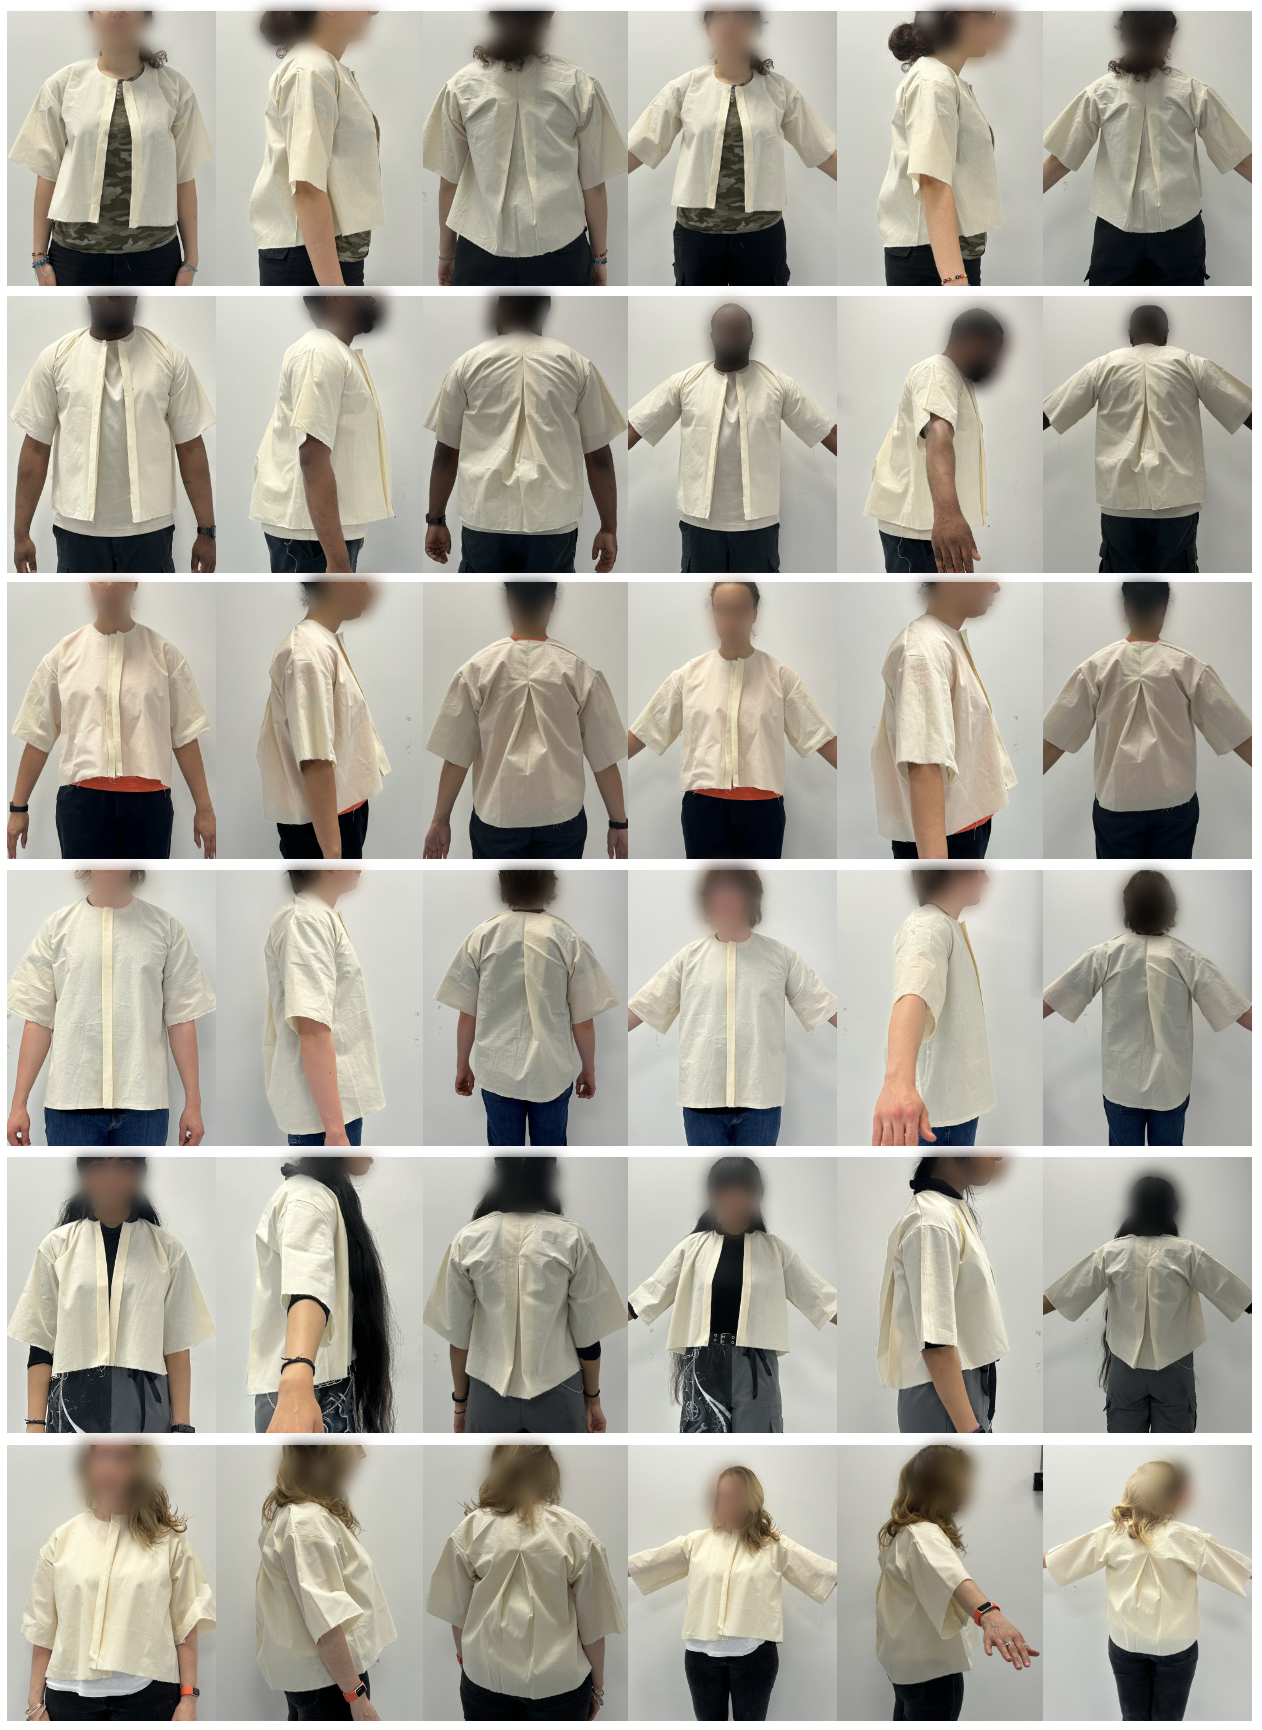
\includegraphics[width = \textwidth]{Images/workshop garments.png}
    \caption{Workshop study garments}
    \label{fig:workshop_garments}
\end{figure}

\begin{figure}[H]
    \centering
    \begin{subfigure}[b]{0.45\textwidth}
        \centering
        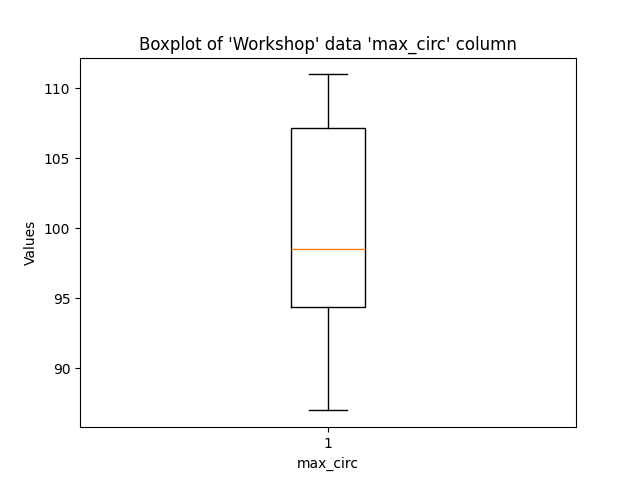
\includegraphics[width=\textwidth]{Images/Workshop_max_circ_Boxplot.png}
        \caption{Max bodice circumference}
        \label{fig:workshop_max_circ}
    \end{subfigure}
    \hfill
    \begin{subfigure}[b]{0.45\textwidth}
        \centering
        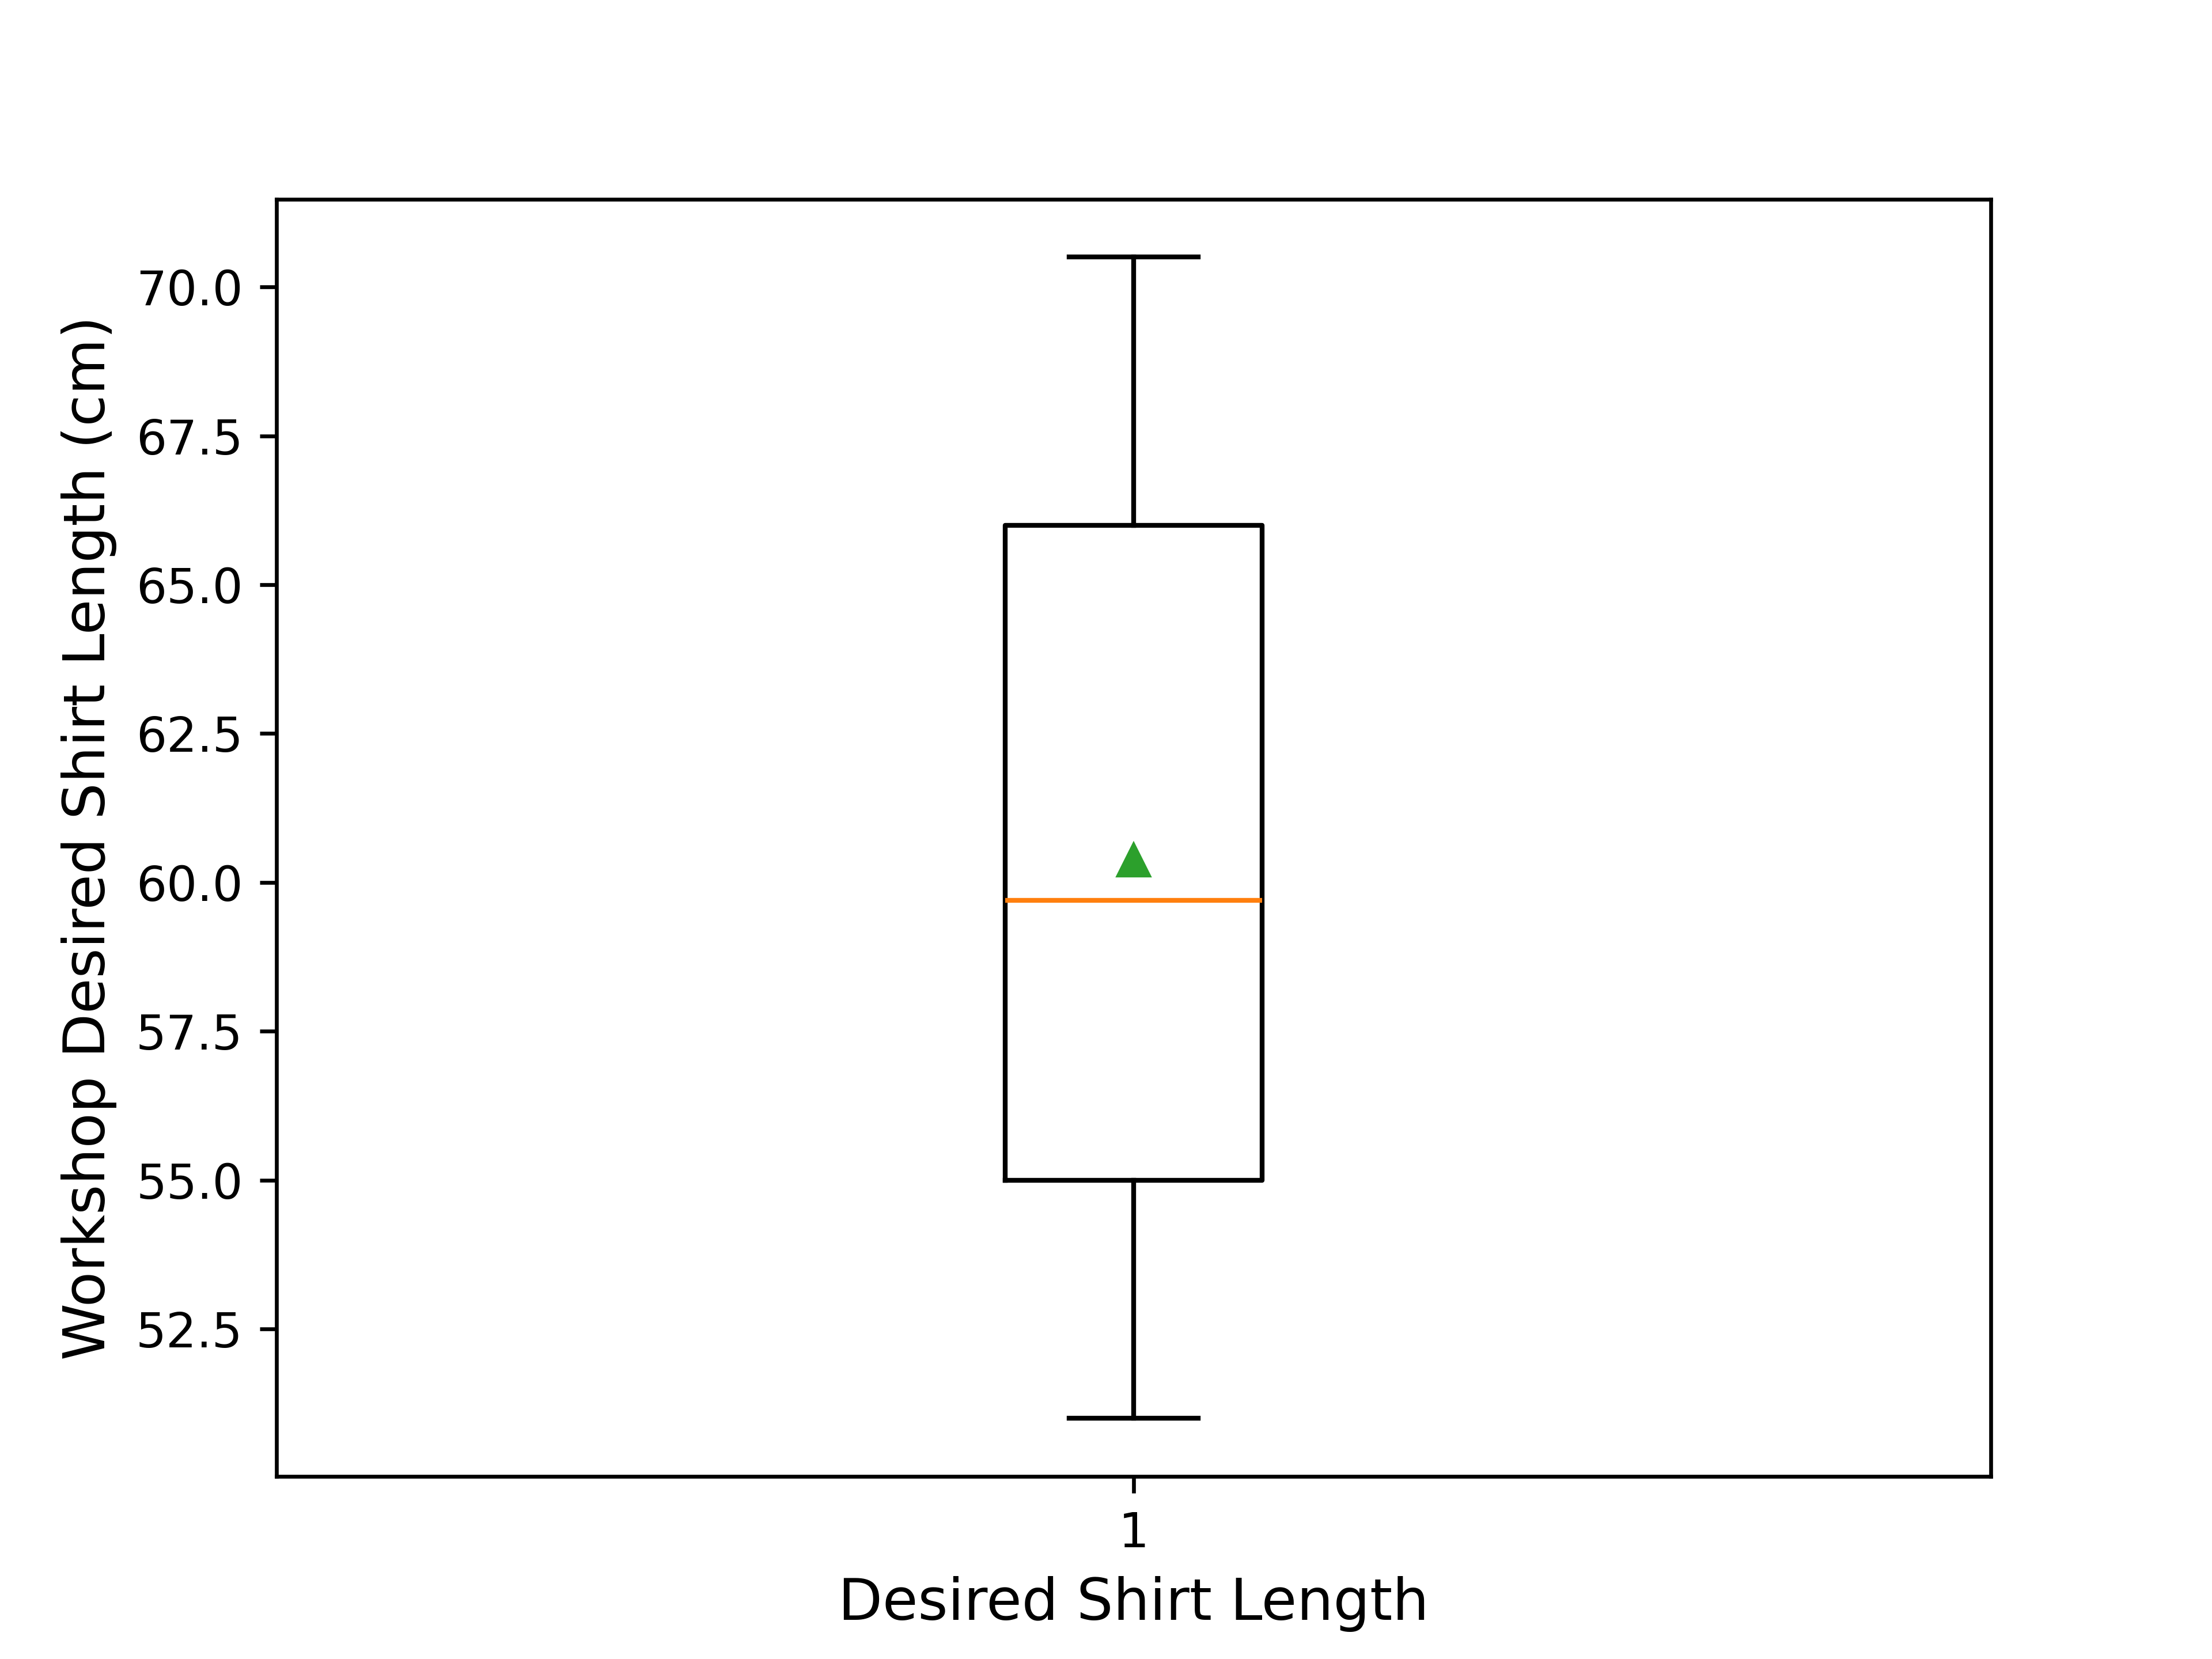
\includegraphics[width=\textwidth]{Images/Workshop_desired_shirt_length_Boxplot.png}
        \caption{Shirt length}
        \label{fig:workshop_shirt_length}
    \end{subfigure}
    \caption{Workshop participant input measurement boxplots}
\end{figure}

\begin{figure}[H]
    \centering
    \begin{subfigure}[b]{0.45\textwidth}
        \centering
        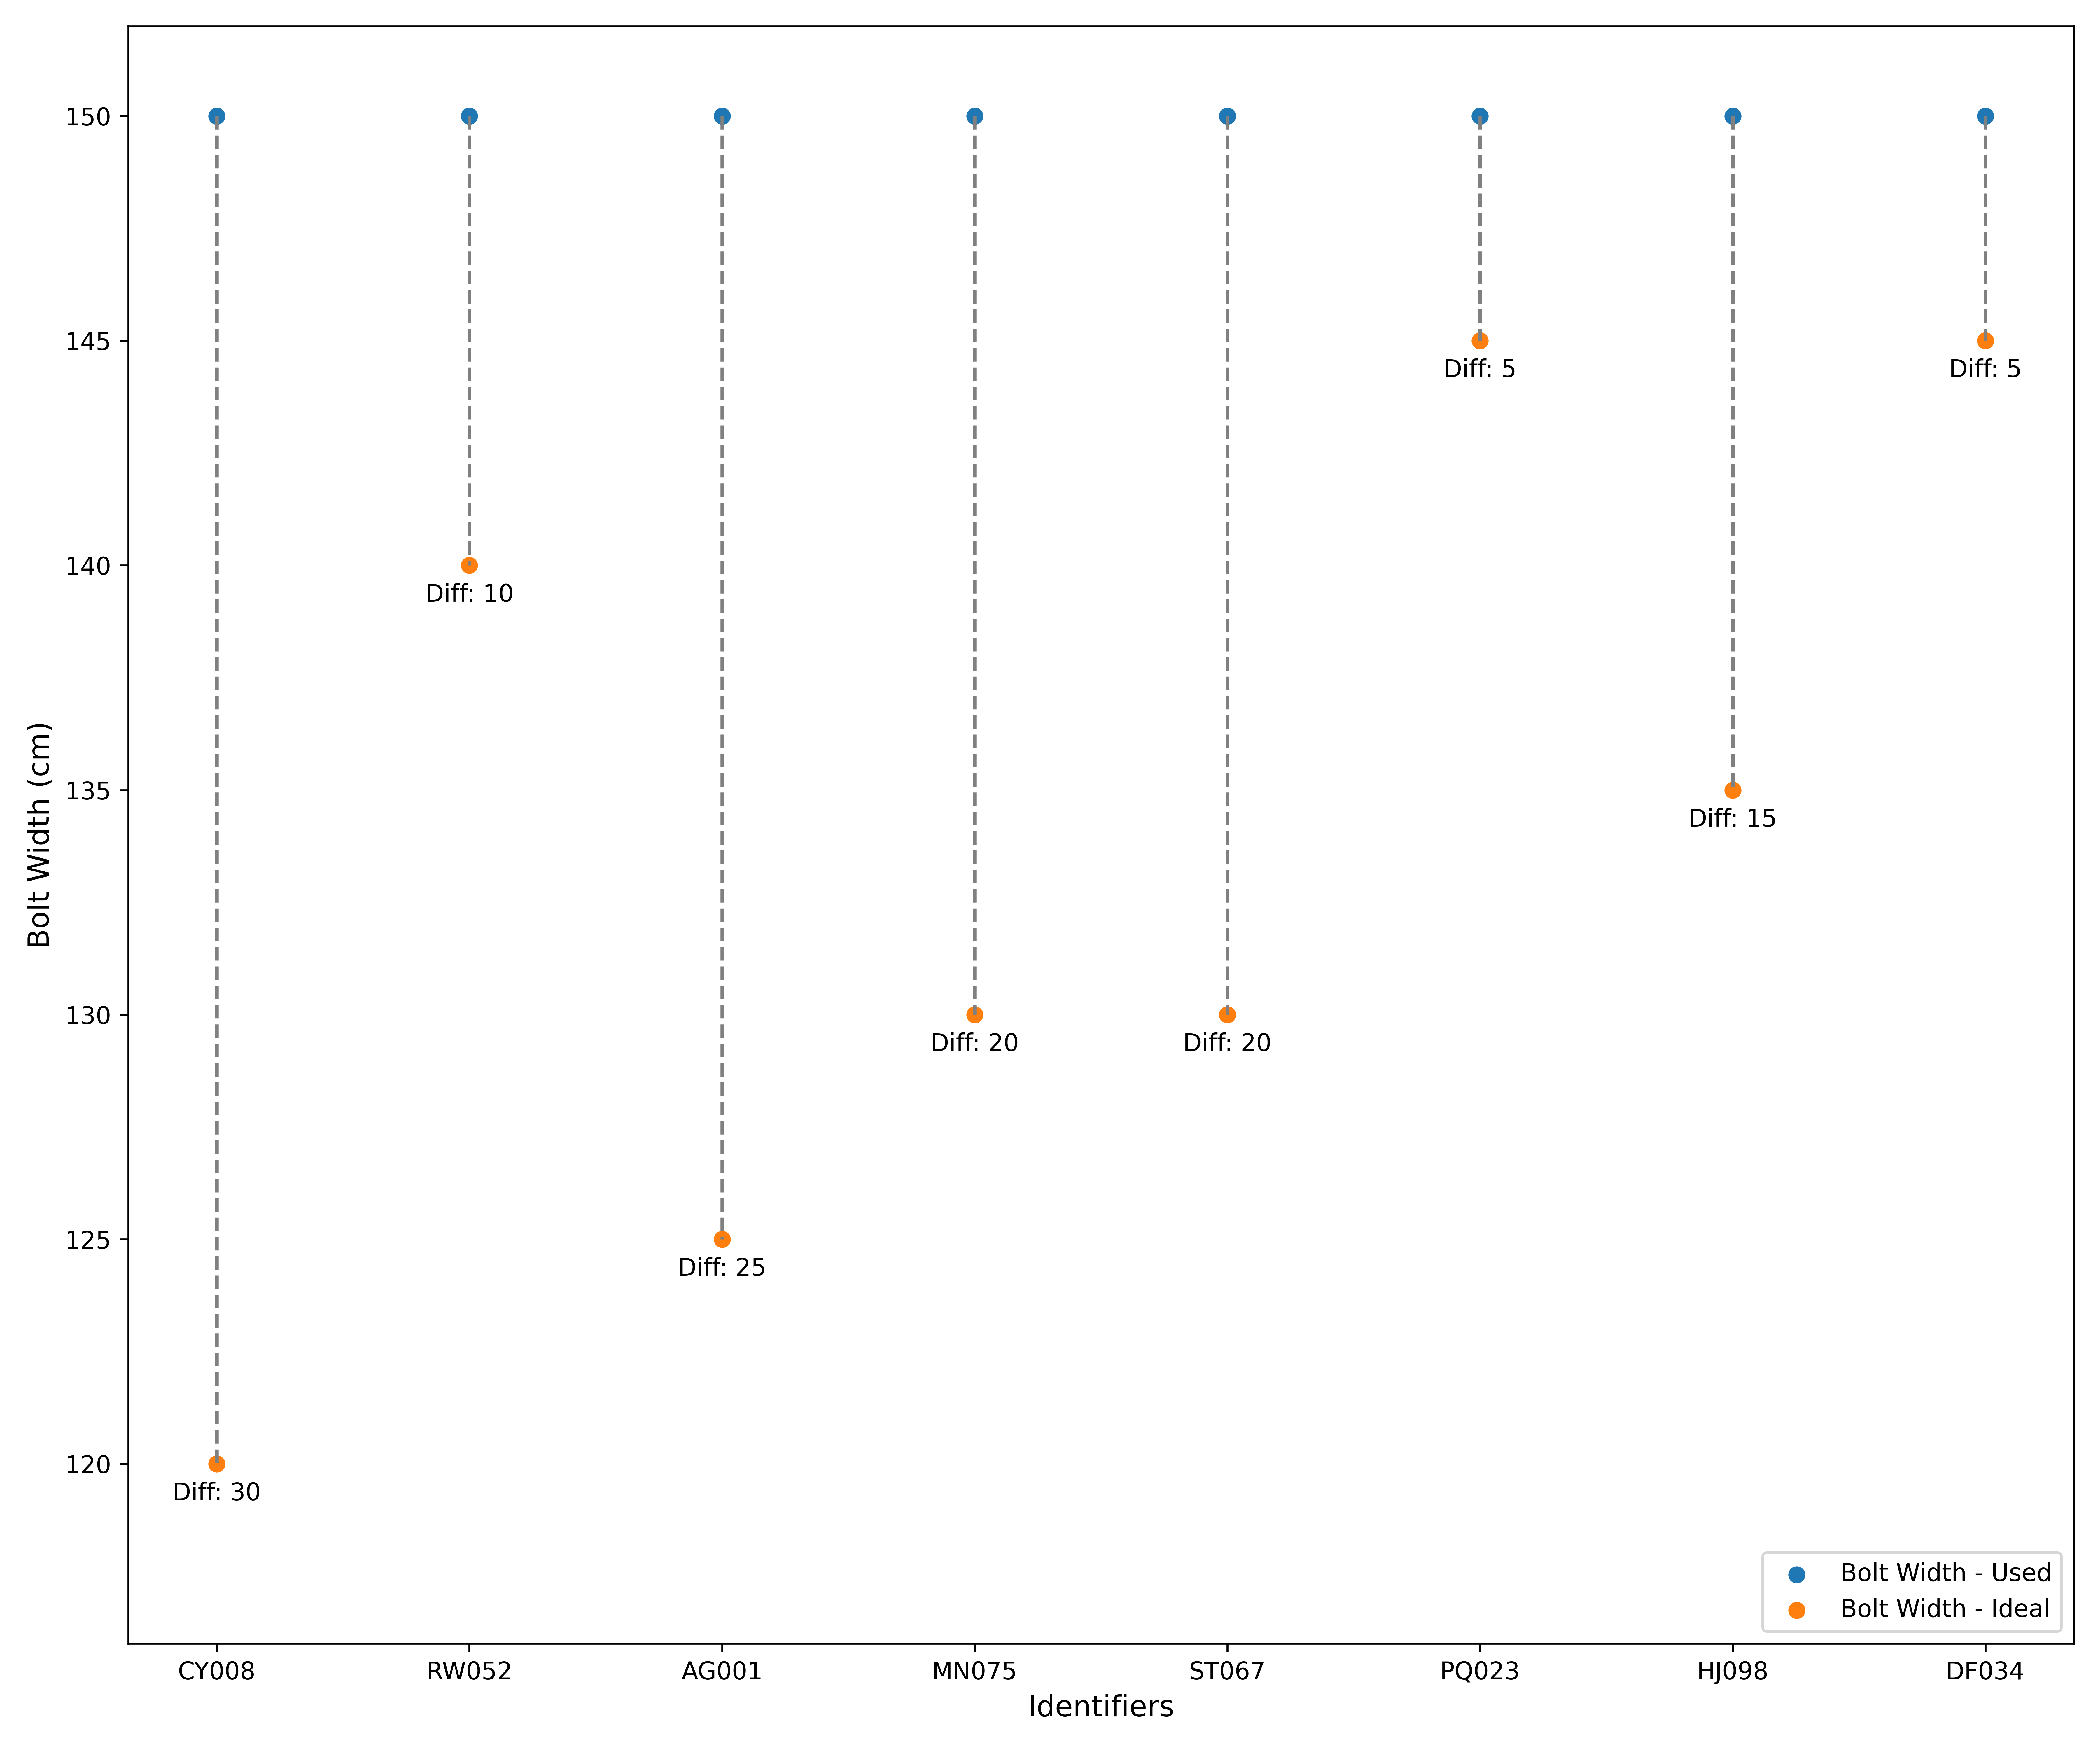
\includegraphics[width=\textwidth]{Images/Workshop_BoltWidths_Scatter.png}
        \caption{}
        \label{fig:workshop_bolt_widths}
    \end{subfigure}
    \vfill
    \begin{subfigure}[b]{0.45\textwidth}
        \centering
        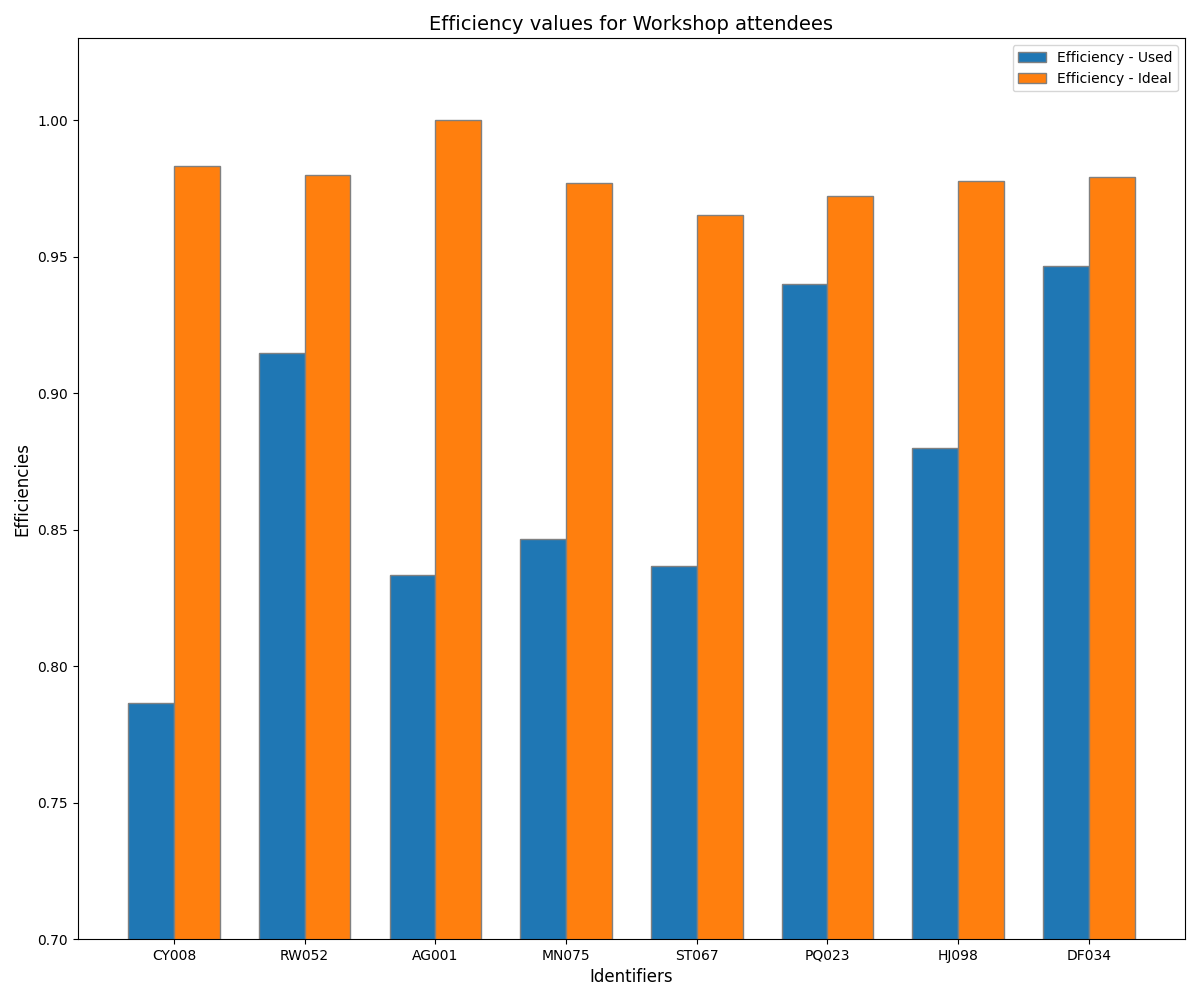
\includegraphics[width=\textwidth]{Images/Workshop_Eff_bar.png}
        \caption{}
        \label{fig:workshop_efficiency_bar}
    \end{subfigure}
    \caption{Workshop ideal vs used bolt widths (a) and efficiencies (b)}
\end{figure}

\begin{figure}[H]
    \centering
    \begin{subfigure}[b]{0.45\textwidth}
        \centering
        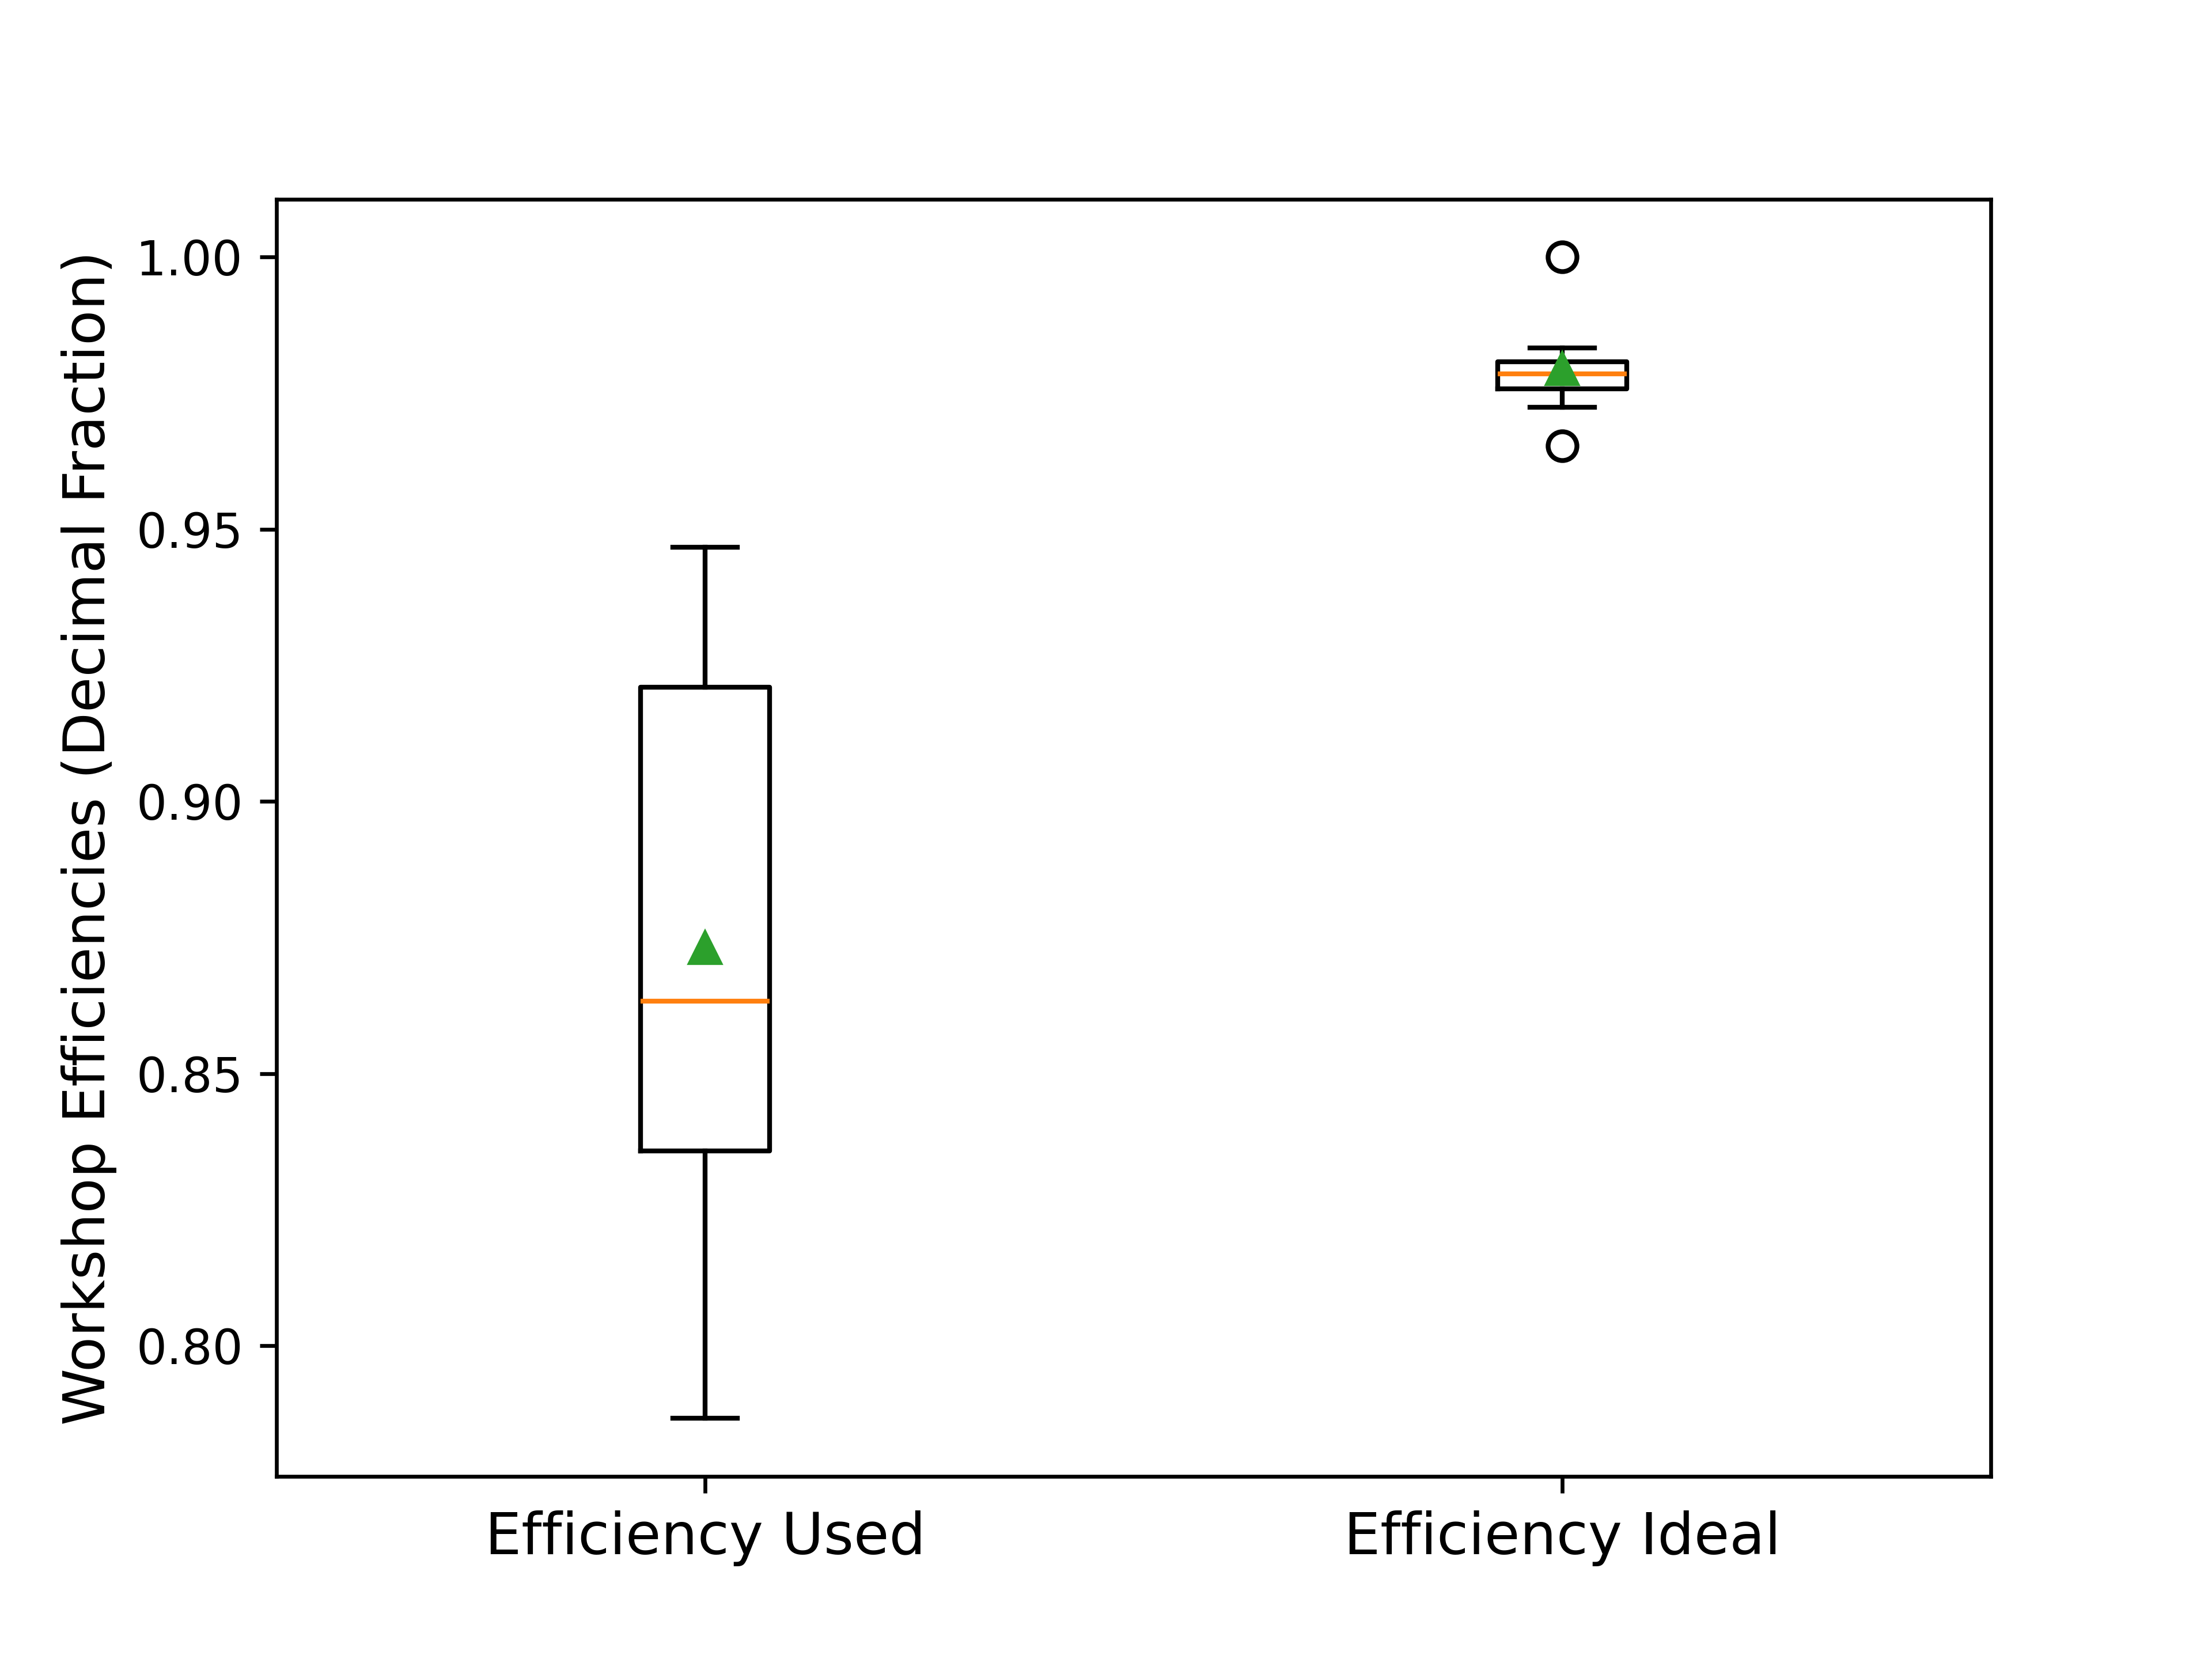
\includegraphics[width=\textwidth]{Images/Workshop Efficiencies_Boxplot.png}
        \caption{}
        \label{fig:workshop_efficiency_boxplot}
    \end{subfigure}
    \begin{subfigure}[b]{0.45\textwidth}
        \centering
        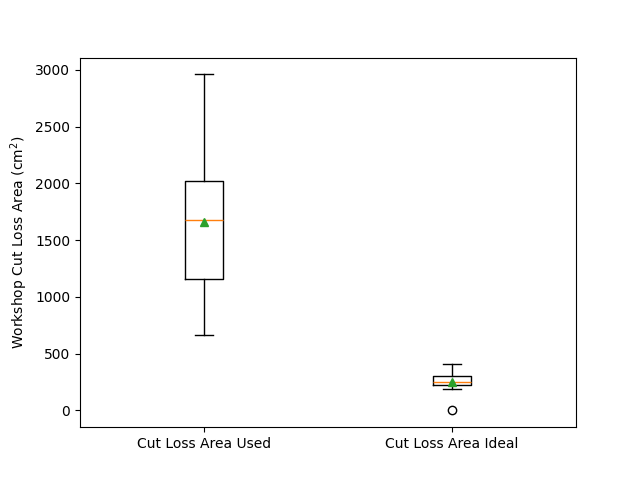
\includegraphics[width=\textwidth]{Images/Workshop Cut Loss Area_Boxplot.png}
        \caption{}
        \label{fig:workshop_cut_loss_area}
    \end{subfigure}
    \caption{}
\end{figure}

Lastly, responses to the Likert scales are graphed (Figures \ref{fig:fit_likert} and \ref{fig:comfort_likert}), showing the qualititative analysis of the participants' satisfaction with the fit and cofort of their finished garments.

\begin{figure} [H]
    \centering
    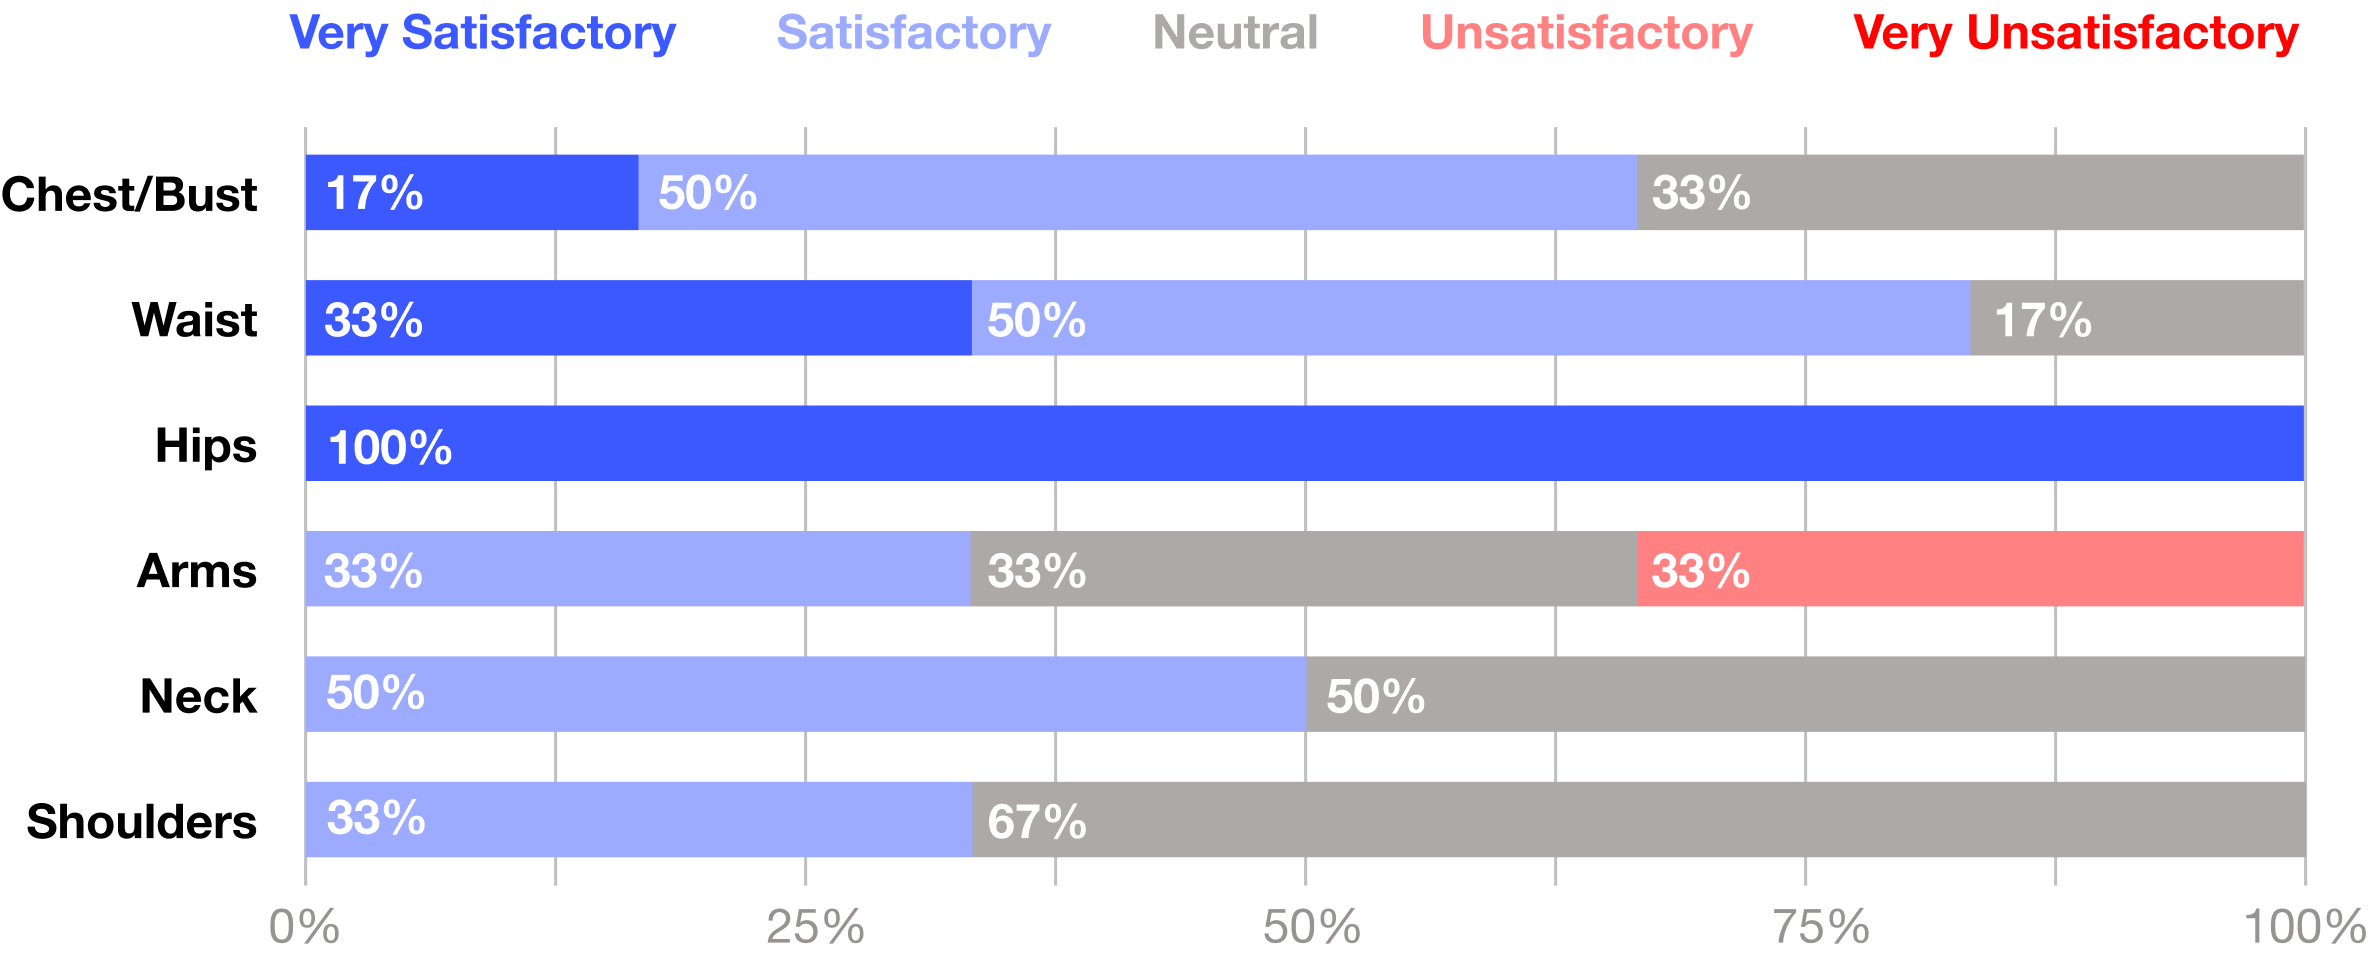
\includegraphics[width = 0.8\textwidth]{Images/fit likert stacked bar.png}
    \caption{Fit Likert Scales}
    \label{fig:fit_likert}
\end{figure}
\begin{figure} [H]
    \centering
    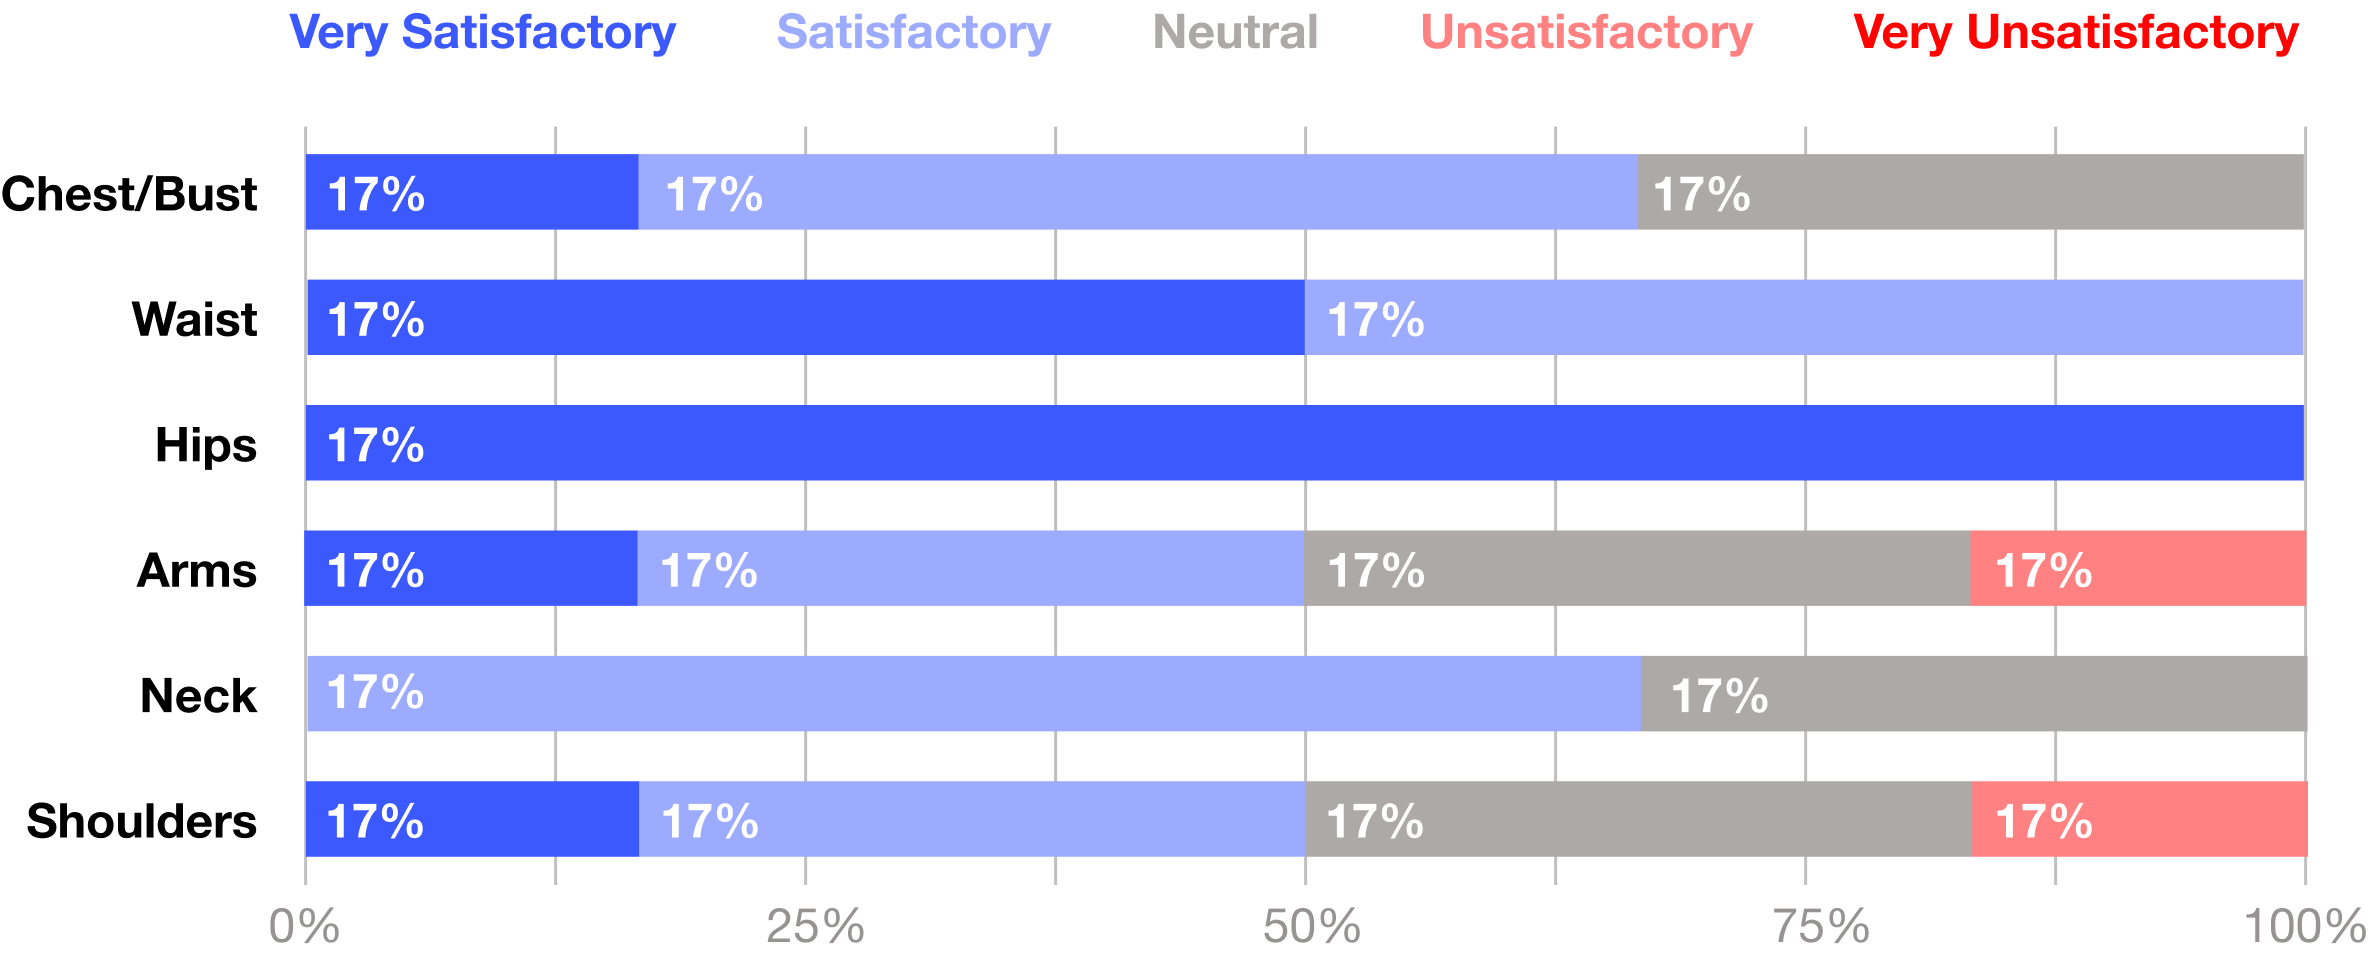
\includegraphics[width = 0.8\textwidth]{Images/comfort likert stacked bar.png}
    \caption{Comfort Likert Scales}
    \label{fig:comfort_likert}
\end{figure}


\section{Body Scans Study}
The body scans study had 100 participants. 

They had a mean maximum bodice circumference of 99.58 cm, median of 98.25 cm and a standard deviation of 8.61 cm (Fig R.10). The mean and median are close, indicating a relatively symmetrical distribution with a slight skew towards larger values. There is moderate variability (standard deviation of 8.613), with some outliers above 110 cm. The mean shirt length is 62.40 cm, median of 64.5 cm, and a standard deviation of 6.72 cm (Fig R.11).

The distributions of ideal efficiencies, bolt width, cut loss areas, cut loss widths are shown in Figures \ref{fig:body_scan_efficiency}, \ref{fig:body_scan_bolt_width}, \ref{fig:body_scan_cut_loss_area}, and \ref{fig:body_scan_cut_loss_width}.

\begin{figure}[H]
    \centering
    \begin{subfigure}[b]{0.45\textwidth}
        \centering
        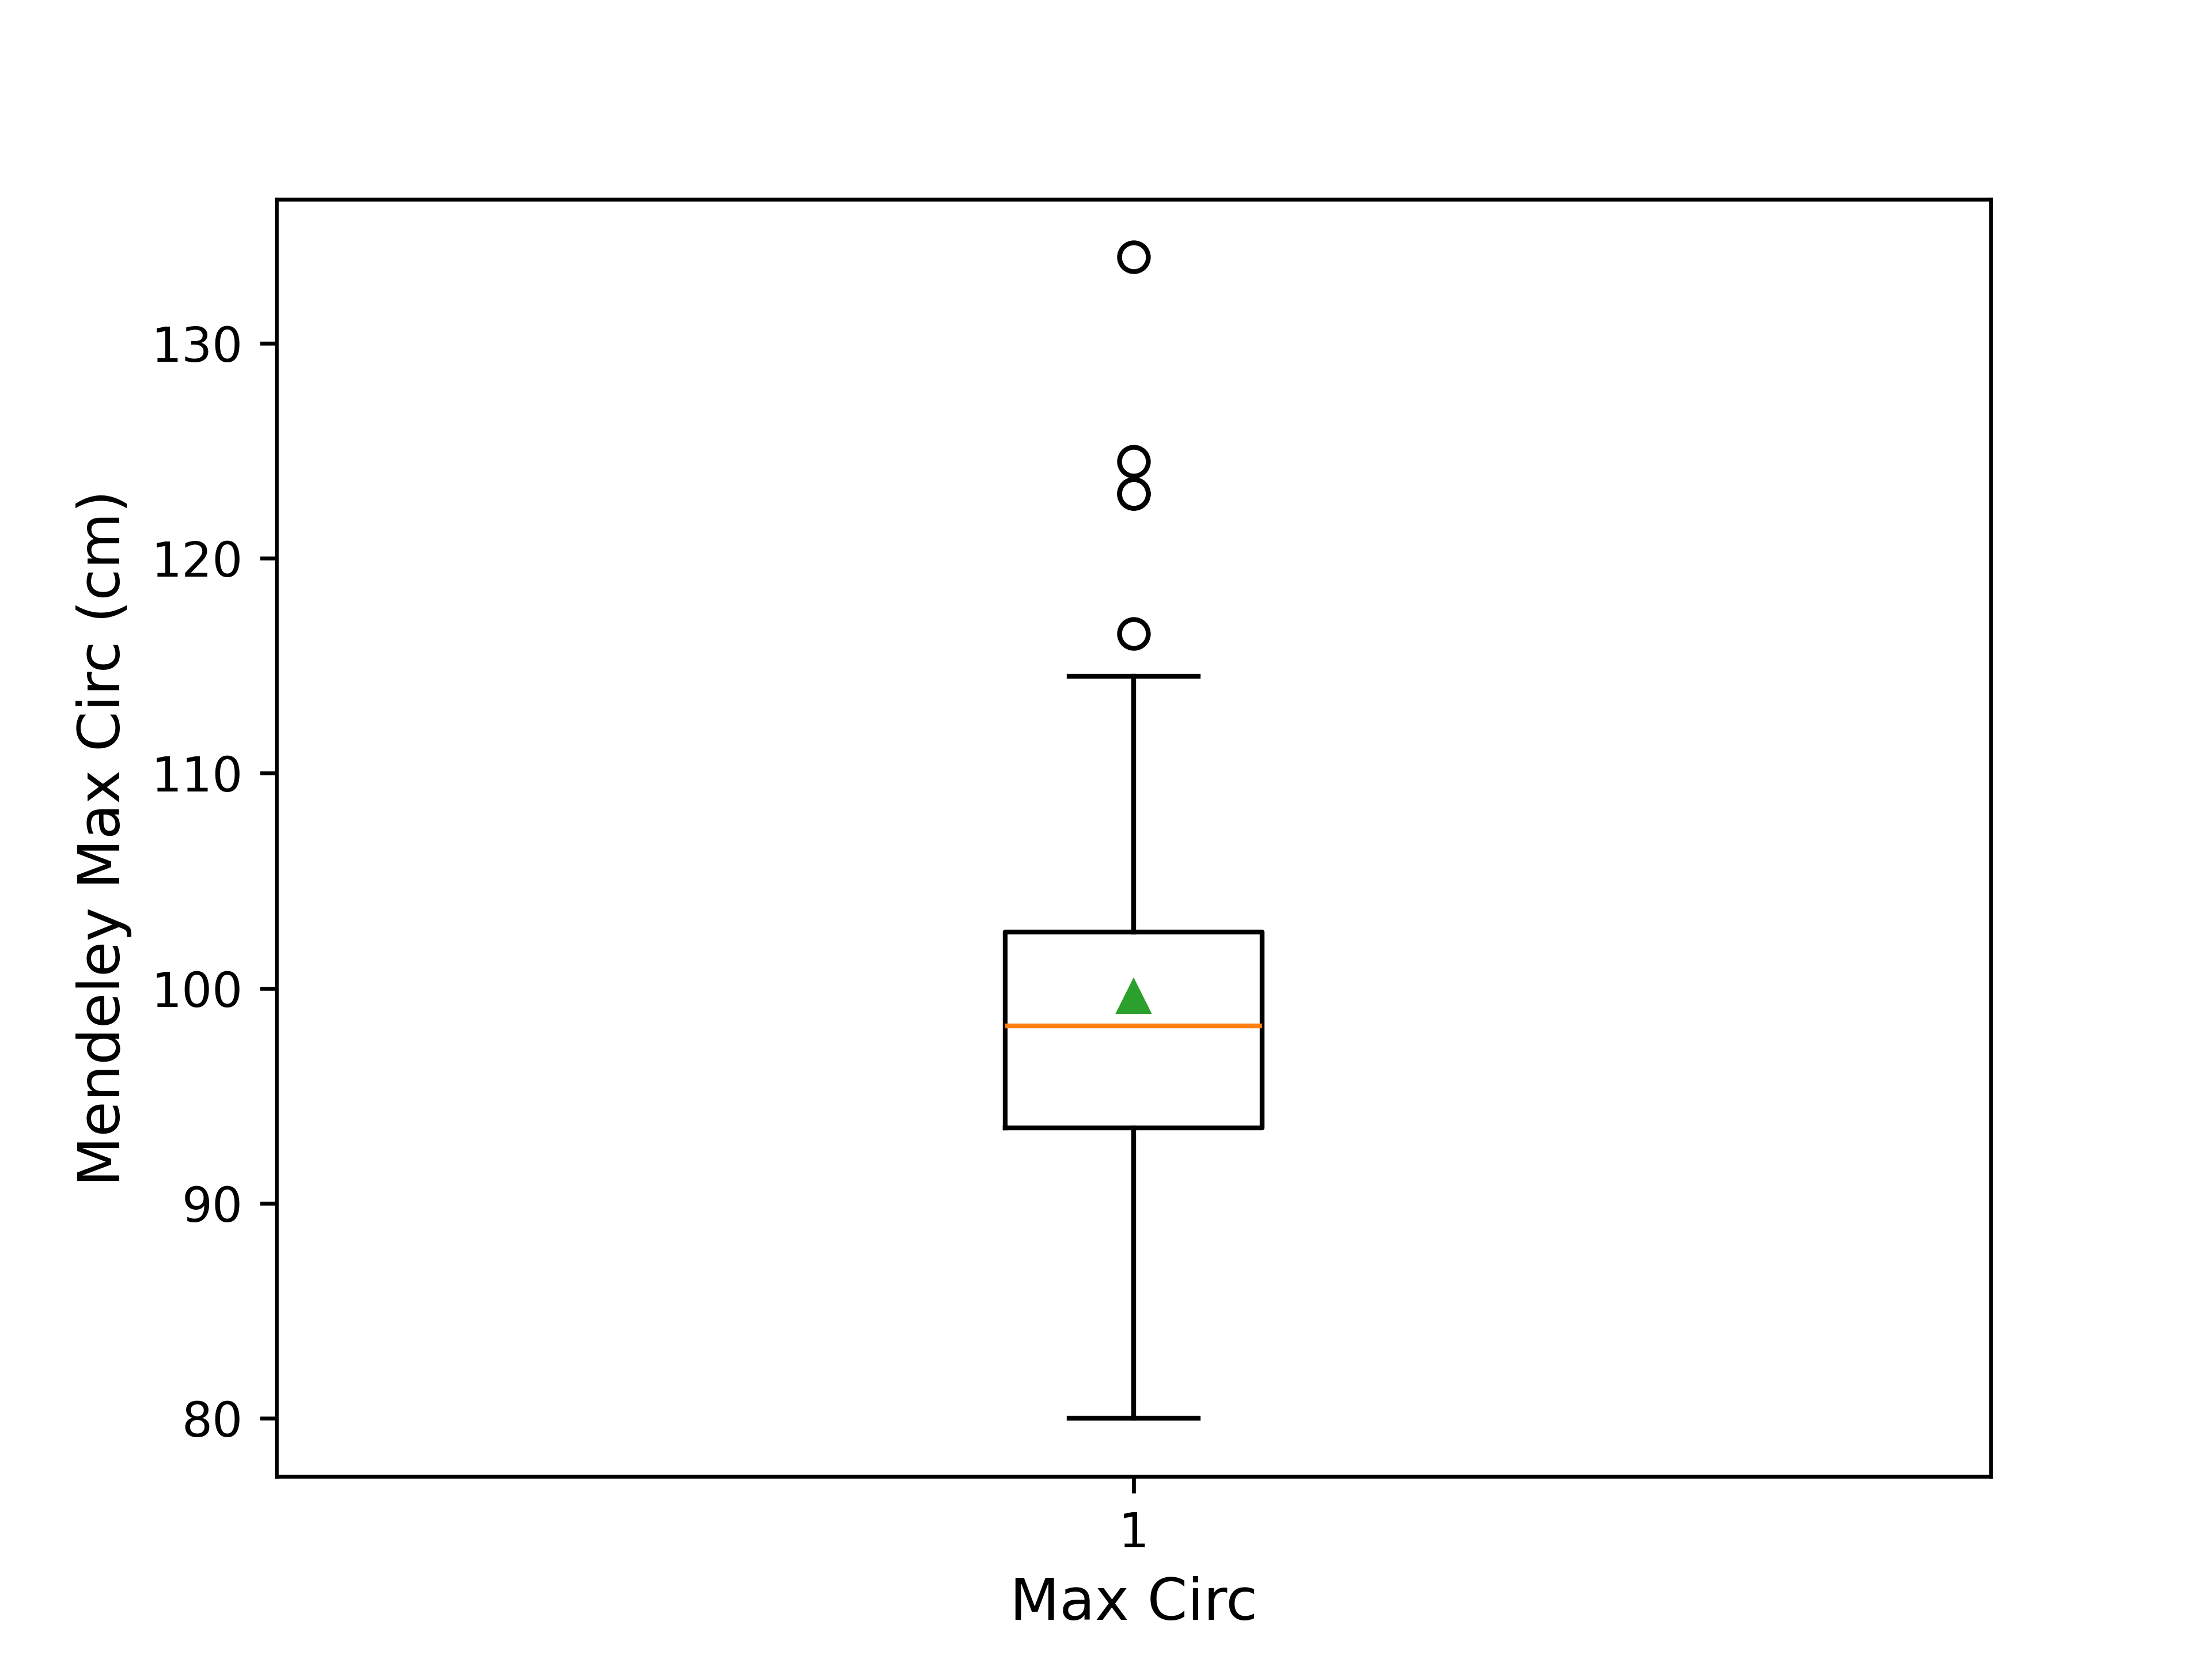
\includegraphics[width=\textwidth]{Images/Mendeley_max_circ_Boxplot.png}
        \caption{Max bodice circumference}
        \label{fig:body_scan_max_circ}
    \end{subfigure}
    \hfill
    \begin{subfigure}[b]{0.45\textwidth}
        \centering
        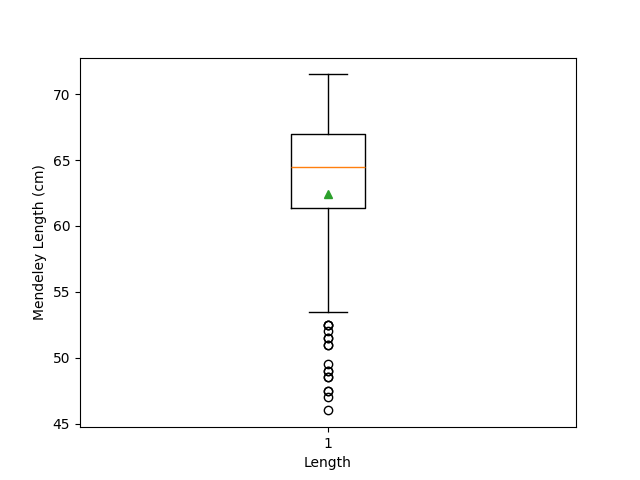
\includegraphics[width=\textwidth]{Images/Mendeley_shirt_length_Boxplot.png}
        \caption{Shirt length}
        \label{fig:body_scan_shirt_length}
    \end{subfigure}
    \caption{Body scan participant input measurement boxplots}
\end{figure}

\begin{figure}[H]
    \centering
    \begin{subfigure}[b]{0.45\textwidth}
        \centering
        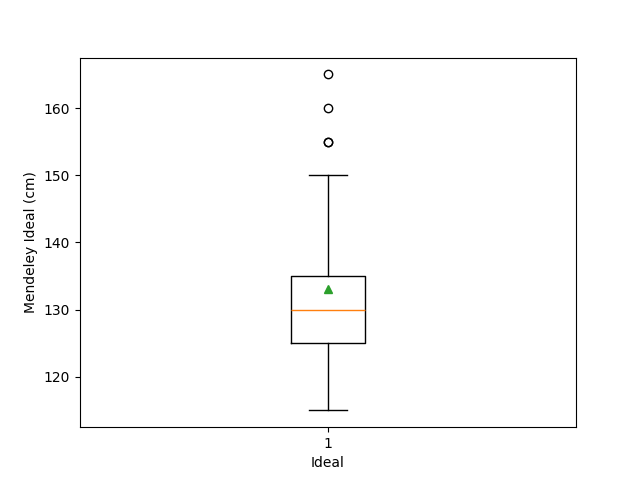
\includegraphics[width=\textwidth]{Images/Mendeley_bolt_width_ideal_Boxplot.png}
        \caption{bolt width}
        \label{fig:body_scan_bolt_width}
    \end{subfigure}
    \hfill
    \begin{subfigure}[b]{0.45\textwidth}
        \centering
        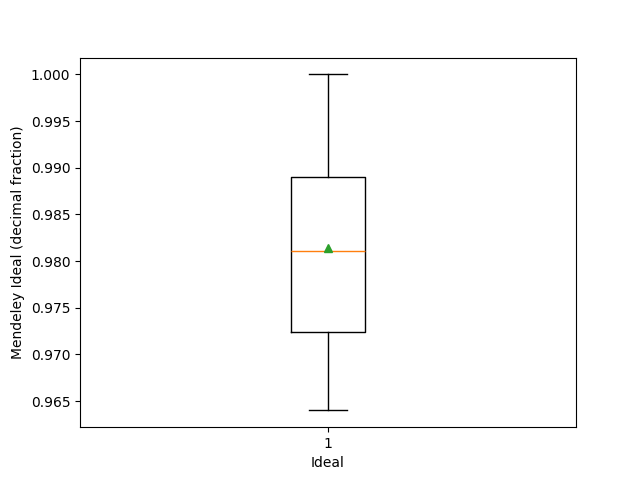
\includegraphics[width=\textwidth]{Images/Mendeley_efficiency_ideal_Boxplot.png}
        \caption{efficiency}
        \label{fig:body_scan_efficiency}
    \end{subfigure}
    \vfill
    \begin{subfigure}[b]{0.45\textwidth}
        \centering
        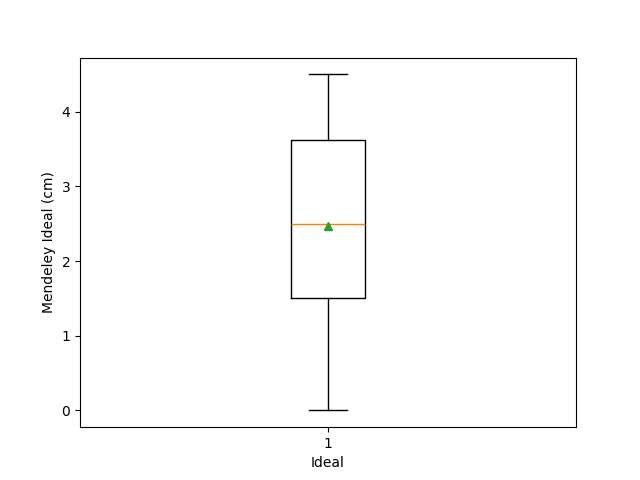
\includegraphics[width=\textwidth]{Images/Mendeley_cut_loss_width_ideal_Boxplot.png}
        \caption{cut loss width}
        \label{fig:body_scan_cut_loss_width}
    \end{subfigure}
    \hfill
    \begin{subfigure}[b]{0.45\textwidth}
        \centering
        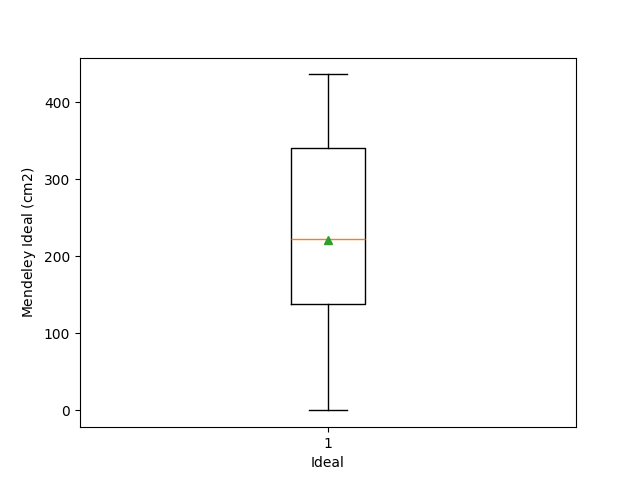
\includegraphics[width=\textwidth]{Images/Mendeley_cut_loss_area_ideal_Boxplot.png}
        \caption{cut loss area}
        \label{fig:body_scan_cut_loss_area}
    \end{subfigure}
    \vfill
    \caption{Body scan ideal case metrics}
\end{figure}
Distributions of cut loss area, efficiency, and embellishment recouped were computed for a range of bolt widths. Data is present in Table \ref{tab:cohort_analysis} and the plotted in Figures (R.16, R.17, R.18) respectively

\begin{table}[H]
    \centering
    \captionsetup{font=small}
    \begin{tabular}{
        >{\centering\arraybackslash}p{1.2cm} | 
        >{\centering\arraybackslash}p{1.5cm} | 
        >{\centering\arraybackslash}p{1.5cm} | 
        >{\centering\arraybackslash}p{1.5cm} | 
        >{\centering\arraybackslash}p{2.2cm} | 
        >{\centering\arraybackslash}p{2.2cm} | 
        >{\centering\arraybackslash}p{2.2cm}
    }
        \toprule
        \textbf{Bolt Width} & \textbf{Mean Eff} & \textbf{Median Eff} & \textbf{St Dev Eff} & \textbf{Mean Loss Area} & \textbf{Median Loss Area} & \textbf{St Dev Loss Area} \\
        \midrule
        110 & 81.7\% & 83.6\% & 6.1\% & 2620.64 & 2318.0 & 889.32 \\
        115 & 78.5\% & 80.0\% & 6.0\% & 3233.87 & 2922.75 & 937.46 \\
        120 & 76.2\% & 77.1\% & 7.4\% & 3737.44 & 3556.88 & 1207.17 \\
        125 & 78.7\% & 75.6\% & 12.1\% & 3526.84 & 4025.0 & 2097.15 \\
        130 & 83.7\% & 91.7\% & 13.5\% & 2771.99 & 934.5 & 2542.75 \\
        135 & 87.9\% & 92.9\% & 12.3\% & 1997.82 & 843.0 & 2501.29 \\
        140 & 88.8\% & 91.1\% & 9.2\% & 1716.44 & 1131.0 & 2025.64 \\
        145 & 87.3\% & 88.1\% & 8.1\% & 1865.09 & 1491.63 & 1849.15 \\
        150 & 85.2\% & 85.5\% & 7.1\% & 2158.84 & 1890.75 & 1679.22 \\
        155 & 83.3\% & 83.1\% & 6.2\% & 2418.42 & 2333.63 & 1388.62 \\
        160 & 81.2\% & 80.6\% & 5.4\% & 2752.84 & 2795.13 & 1076.74 \\
        165 & 79.1\% & 78.3\% & 5.2\% & 3089.52 & 3250.13 & 782.20 \\
        \bottomrule
    \end{tabular}
    \caption{Description of Cohort Analysis on Different Bolts for 100 Scans Study}
    \label{tab:cohort_analysis}
\end{table}

\begin{figure}[H]
    \centering
    \begin{subfigure}[b]{0.45\textwidth}
        \centering
        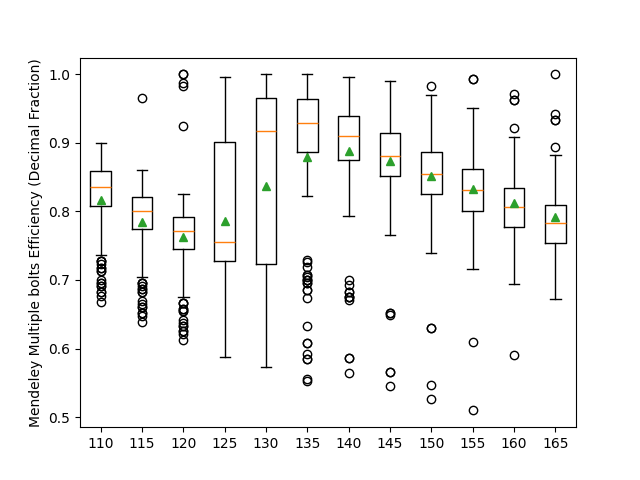
\includegraphics[width=\textwidth]{Images/Mendeley Multiple bolts Efficiency_Boxplot.png}
        \caption{efficiency}
        \label{fig:multibolt_efficiency}
    \end{subfigure}
    \hfill
    \begin{subfigure}[b]{0.45\textwidth}
        \centering
        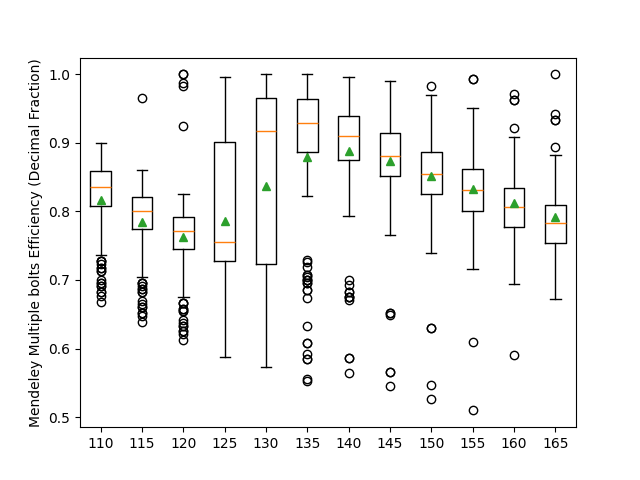
\includegraphics[width=\textwidth]{Images/Mendeley Multiple bolts Efficiency_Boxplot.png}
        \caption{cut loss area}
        \label{fig:multibolt_cut_loss_area}
    \end{subfigure}
    \vfill
    \begin{subfigure}[b]{0.45\textwidth}
        \centering
        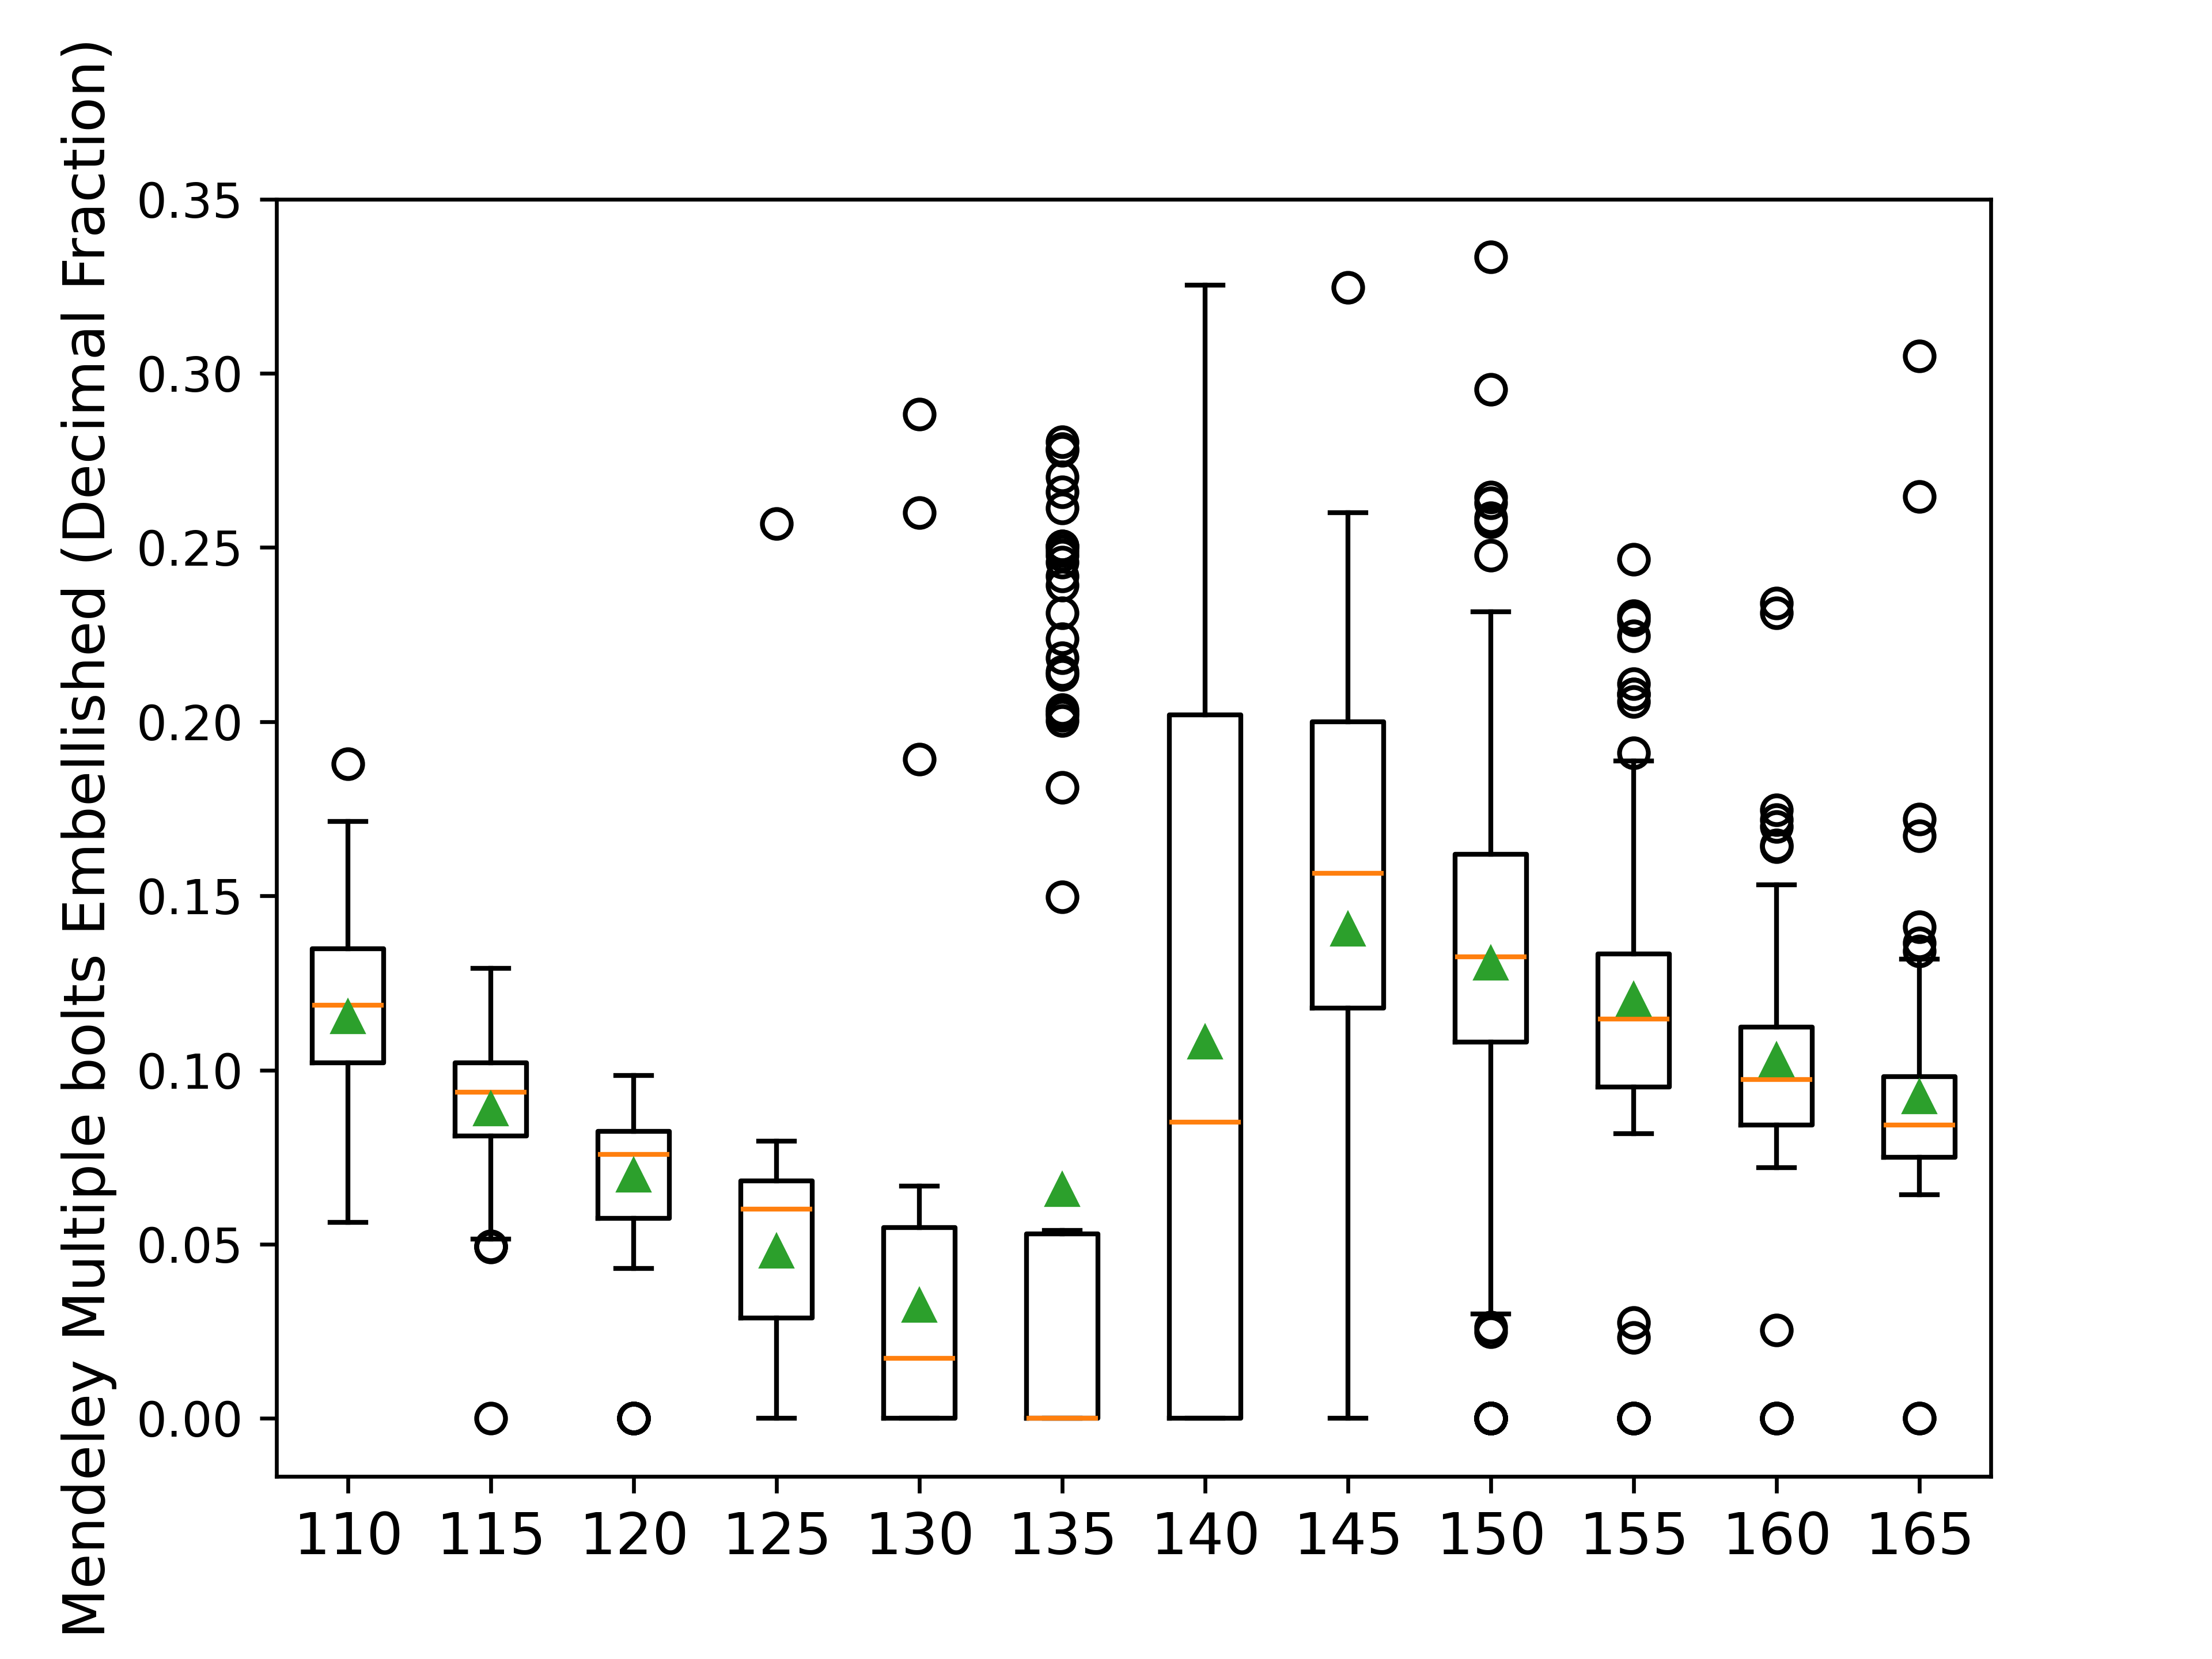
\includegraphics[width=\textwidth]{Images/Mendeley Multiple bolts Embellished_Boxplot.png}
        \caption{embellished}
        \label{multibolt_embellished}
    \end{subfigure}
    \caption{Multiple bolt body scan study cohort analysis}
    \label{fig:multibolt_analysis}
\end{figure}

Count of pattern orientation on starting fabric and possibility of embellishment potential for various bolt widths ranging from 110 to 160 cm.
\begin{figure} [H]
    \centering
    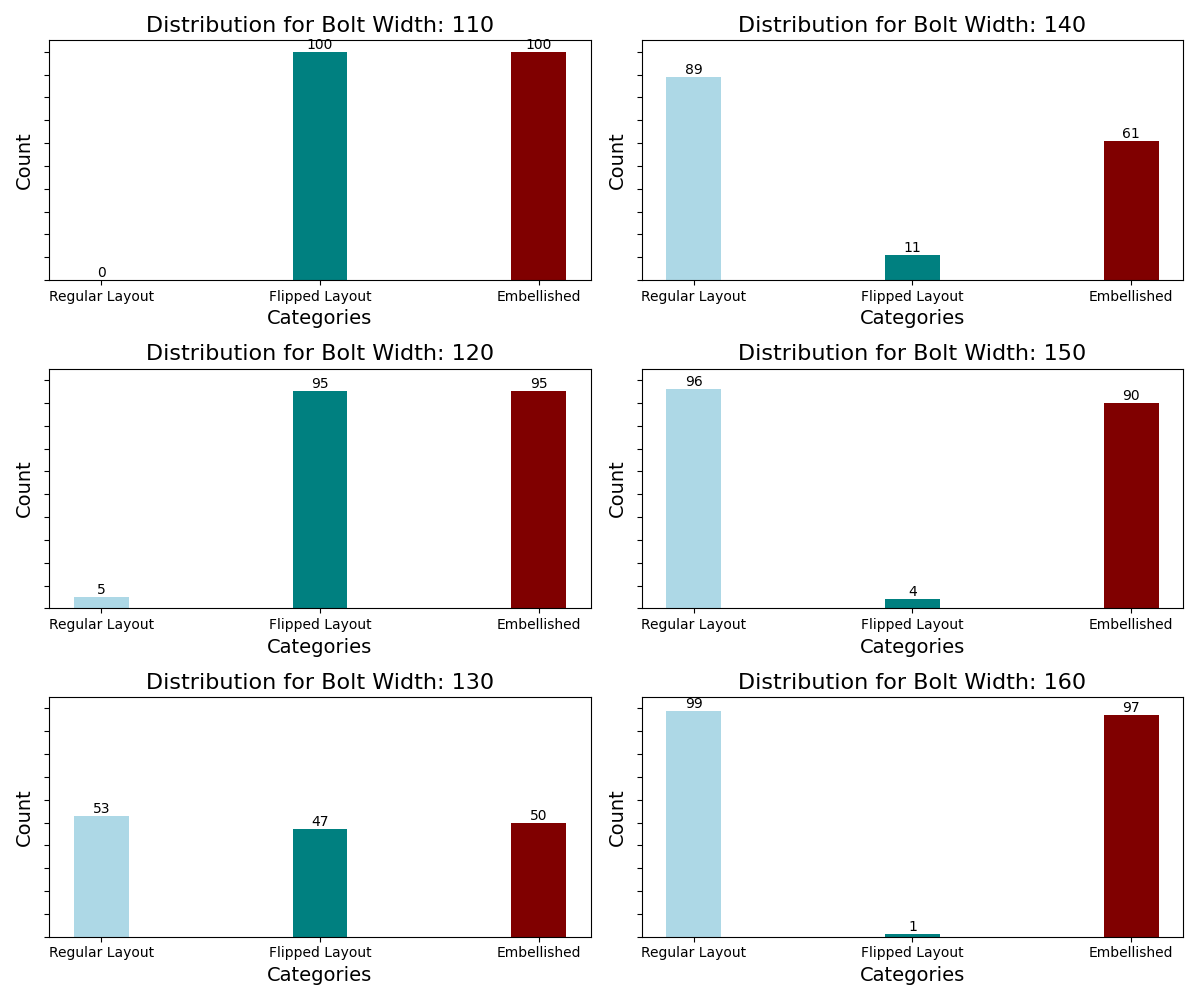
\includegraphics[width = \textwidth]{Images/Mendeley_Bar.png}
    \caption{Layout and Embellishment Possibility for 100 Scans Study}
\end{figure}
For the range of bolt widths between 110 and 160 cm, each pattern generated for the Mendeley dataset participants will fit in the regular or rotated orientation. No mitigation strategies need to be employed within this range of bolts.


\section{Personal Case Study}
Using the parameterisation method defined, the author's pattern width and pattern height is 128.5 cm and 98.5 cm, respectively. The obj file obtained from the 3D scan was imported into CLO3D as the avatar. The pattern pieces were both virtually sewed and draped (Figure \ref{fig:renderedCLO}) and the physically cut and sewed into the tangible garment (Figure \ref{fig:personal_garment}).

\begin{figure}[H]
    \centering
    \begin{subfigure}[b]{0.3\textwidth}
        \centering
        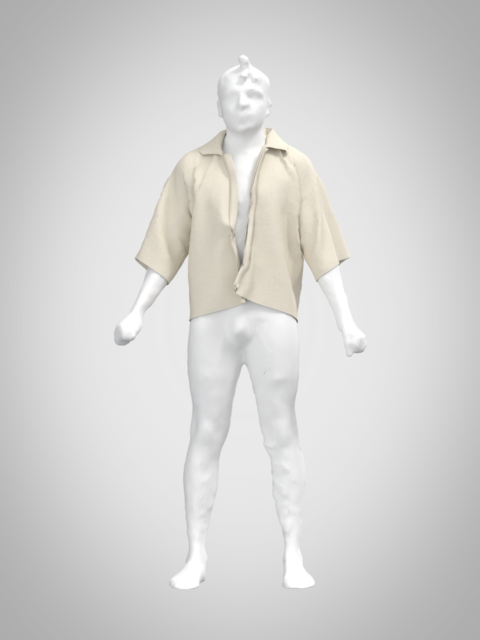
\includegraphics[width=\textwidth]{Images/renderfront.png}
        \caption{Front}
    \end{subfigure}
    \hfill
    \begin{subfigure}[b]{0.3\textwidth}
        \centering
        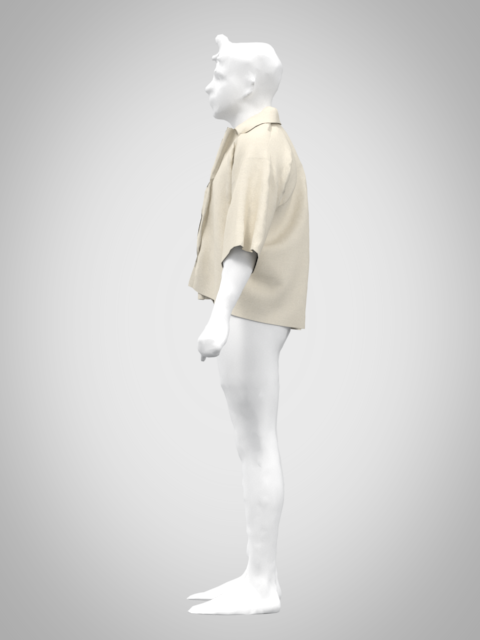
\includegraphics[width=\textwidth]{Images/renderside.png}
        \caption{Side}
    \end{subfigure}
    \hfill
    \begin{subfigure}[b]{0.3\textwidth}
        \centering
        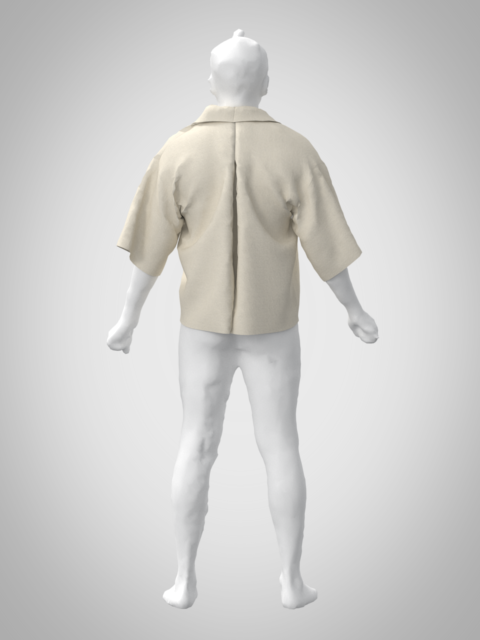
\includegraphics[width=\textwidth]{Images/render backpng.png}
        \caption{Back}
    \end{subfigure}
    \caption{Custom shirt draped on personal scan in CLO3D}
    \label{fig:renderedCLO}
\end{figure}

\begin{figure}[H]
    \centering
    \begin{subfigure}[b]{0.3\textwidth}
        \centering
        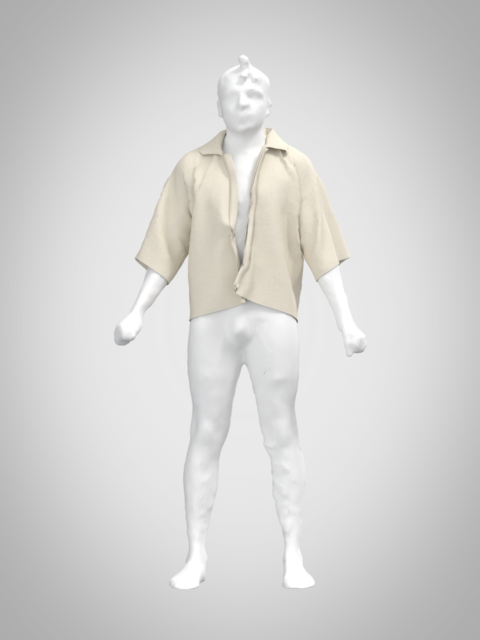
\includegraphics[width=\textwidth]{Images/renderfront.png}
        \caption{Front}
    \end{subfigure}
    \hfill
    \begin{subfigure}[b]{0.3\textwidth}
        \centering
        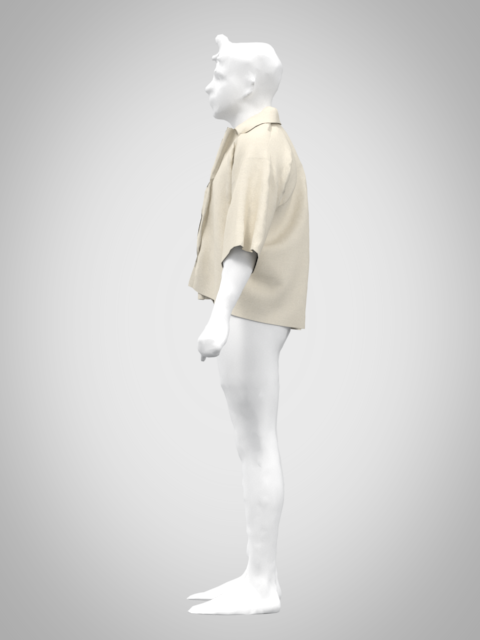
\includegraphics[width=\textwidth]{Images/renderside.png}
        \caption{Side}
    \end{subfigure}
    \hfill
    \begin{subfigure}[b]{0.3\textwidth}
        \centering
        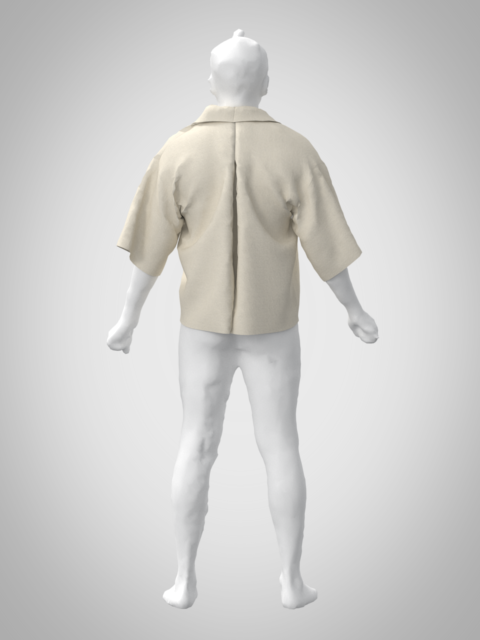
\includegraphics[width=\textwidth]{Images/render backpng.png}
        \caption{Back}
    \end{subfigure}
    \caption{Custom shirt draped on personal scan in CLO3D}
    \label{fig:personal_garment}
\end{figure}